\section{Numerical Experiments}\label{sec:exp} 
In what follows, \Cref{sec:exp1} is themed around the key insight obtained from \Cref{th:main}, i.e., the correlation of the gates lies at the heart of `what is learnt in a DNN with ReLUs'. In particular, we show that operations (such as permuting the layers, tiling cum rotation of the gates, and giving a constant `all-ones' input to the value network) that destroy the layer by layer computational structure do not degrade test performance. These operations lead to combinatorially many models and in all of them the test performance remains the same. In \Cref{sec:exp2} we throw light on the open question in [\citenum{randlabel}] on why test performance degrades due to upstream training with random labels. 
\subsection{Robustness of Gates: Destroying layer-by-layer structure does not affect performance}\label{sec:exp1}
In this experiment we show that information in the gates is invariant even if we destroy the layer-by-layer structure. We consider the three kinds of gates (or gating regimes) described below.\\
\indent \quad$1.$ \textbf{Fixed Learnt:} We \emph{pre-train} the feature network (which is a DNN with ReLUs), then \emph{freeze} the weights of the feature network, and then train the value network. This way we can measure information in the gates of a trained DNN.\\
\indent \quad$2.$ \textbf{Fixed Random:} We initialise the feature network at random, and then \emph{freeze} its weights and then train the value network. This way we can measure information in the gates of a DNN at initialisation. Here, the feature and value network can be either initialised with the same weights i.e., dependent initialisation (DI) or statistically independent weights  i.e., independent initialisation (II).\\
\indent \quad$3.$ \textbf{Decoupled Learning:} We initialise the weights of the value and feature network statistically independent and then train both of them. For the gradient to flow through the feature network we use \emph{soft-gating}, i.e., $G(q)=\frac{1}{1+\exp({-\beta\cdot q})}$, with $\beta=10$. 

We make use of the deep gated network (DGN) setup shown in \Cref{fig:dgn-prior-new} (right) which is an improvisation of the DGN in prior work [\citenum{npk}] shown in \Cref{fig:dgn-prior-new} (left). In the current setup, {\bf{$G_{i_1},\ldots,G_{i_4}$ is a permutation of the $G_1,\ldots,G_4$}}, which gives $24$ models. Note that these \textbf{permutations destroy the layer by layer structure}. In the prior setup both value and feature networks have the same input $x\in\R^{\din}$. In the current setup, we have two separate inputs, $x^{\text{f}}\in\R^{\din}$ for the feature network and $x^{\text{v}}\in\R^{\din}$ for the value network. We set $x^{\text{f}}=x$ always, however, for $x^{\text{v}}$ there are \textbf{two modes} namely (i) \textbf{standard}: we set $x^{\text{v}}=x$ ,(ii) \textbf{`all-ones'}: we set $x^{\text{v}}=\mathbf{1}\in\R^{\din}$ (a tensor of all $1$'s). While the setup on the left is only one model, the setup on the right has $\mathbf{48=24\times 2}$ \textbf{different models}, where $24=\texttt{factorial}(4)$ is due to the gate permutations and $2$ is due the settings of $x^{\text{v}}$.
\begin{figure}[t]
\centering
\begin{minipage}{0.4\columnwidth}
\centering
\resizebox{\columnwidth}{!}{
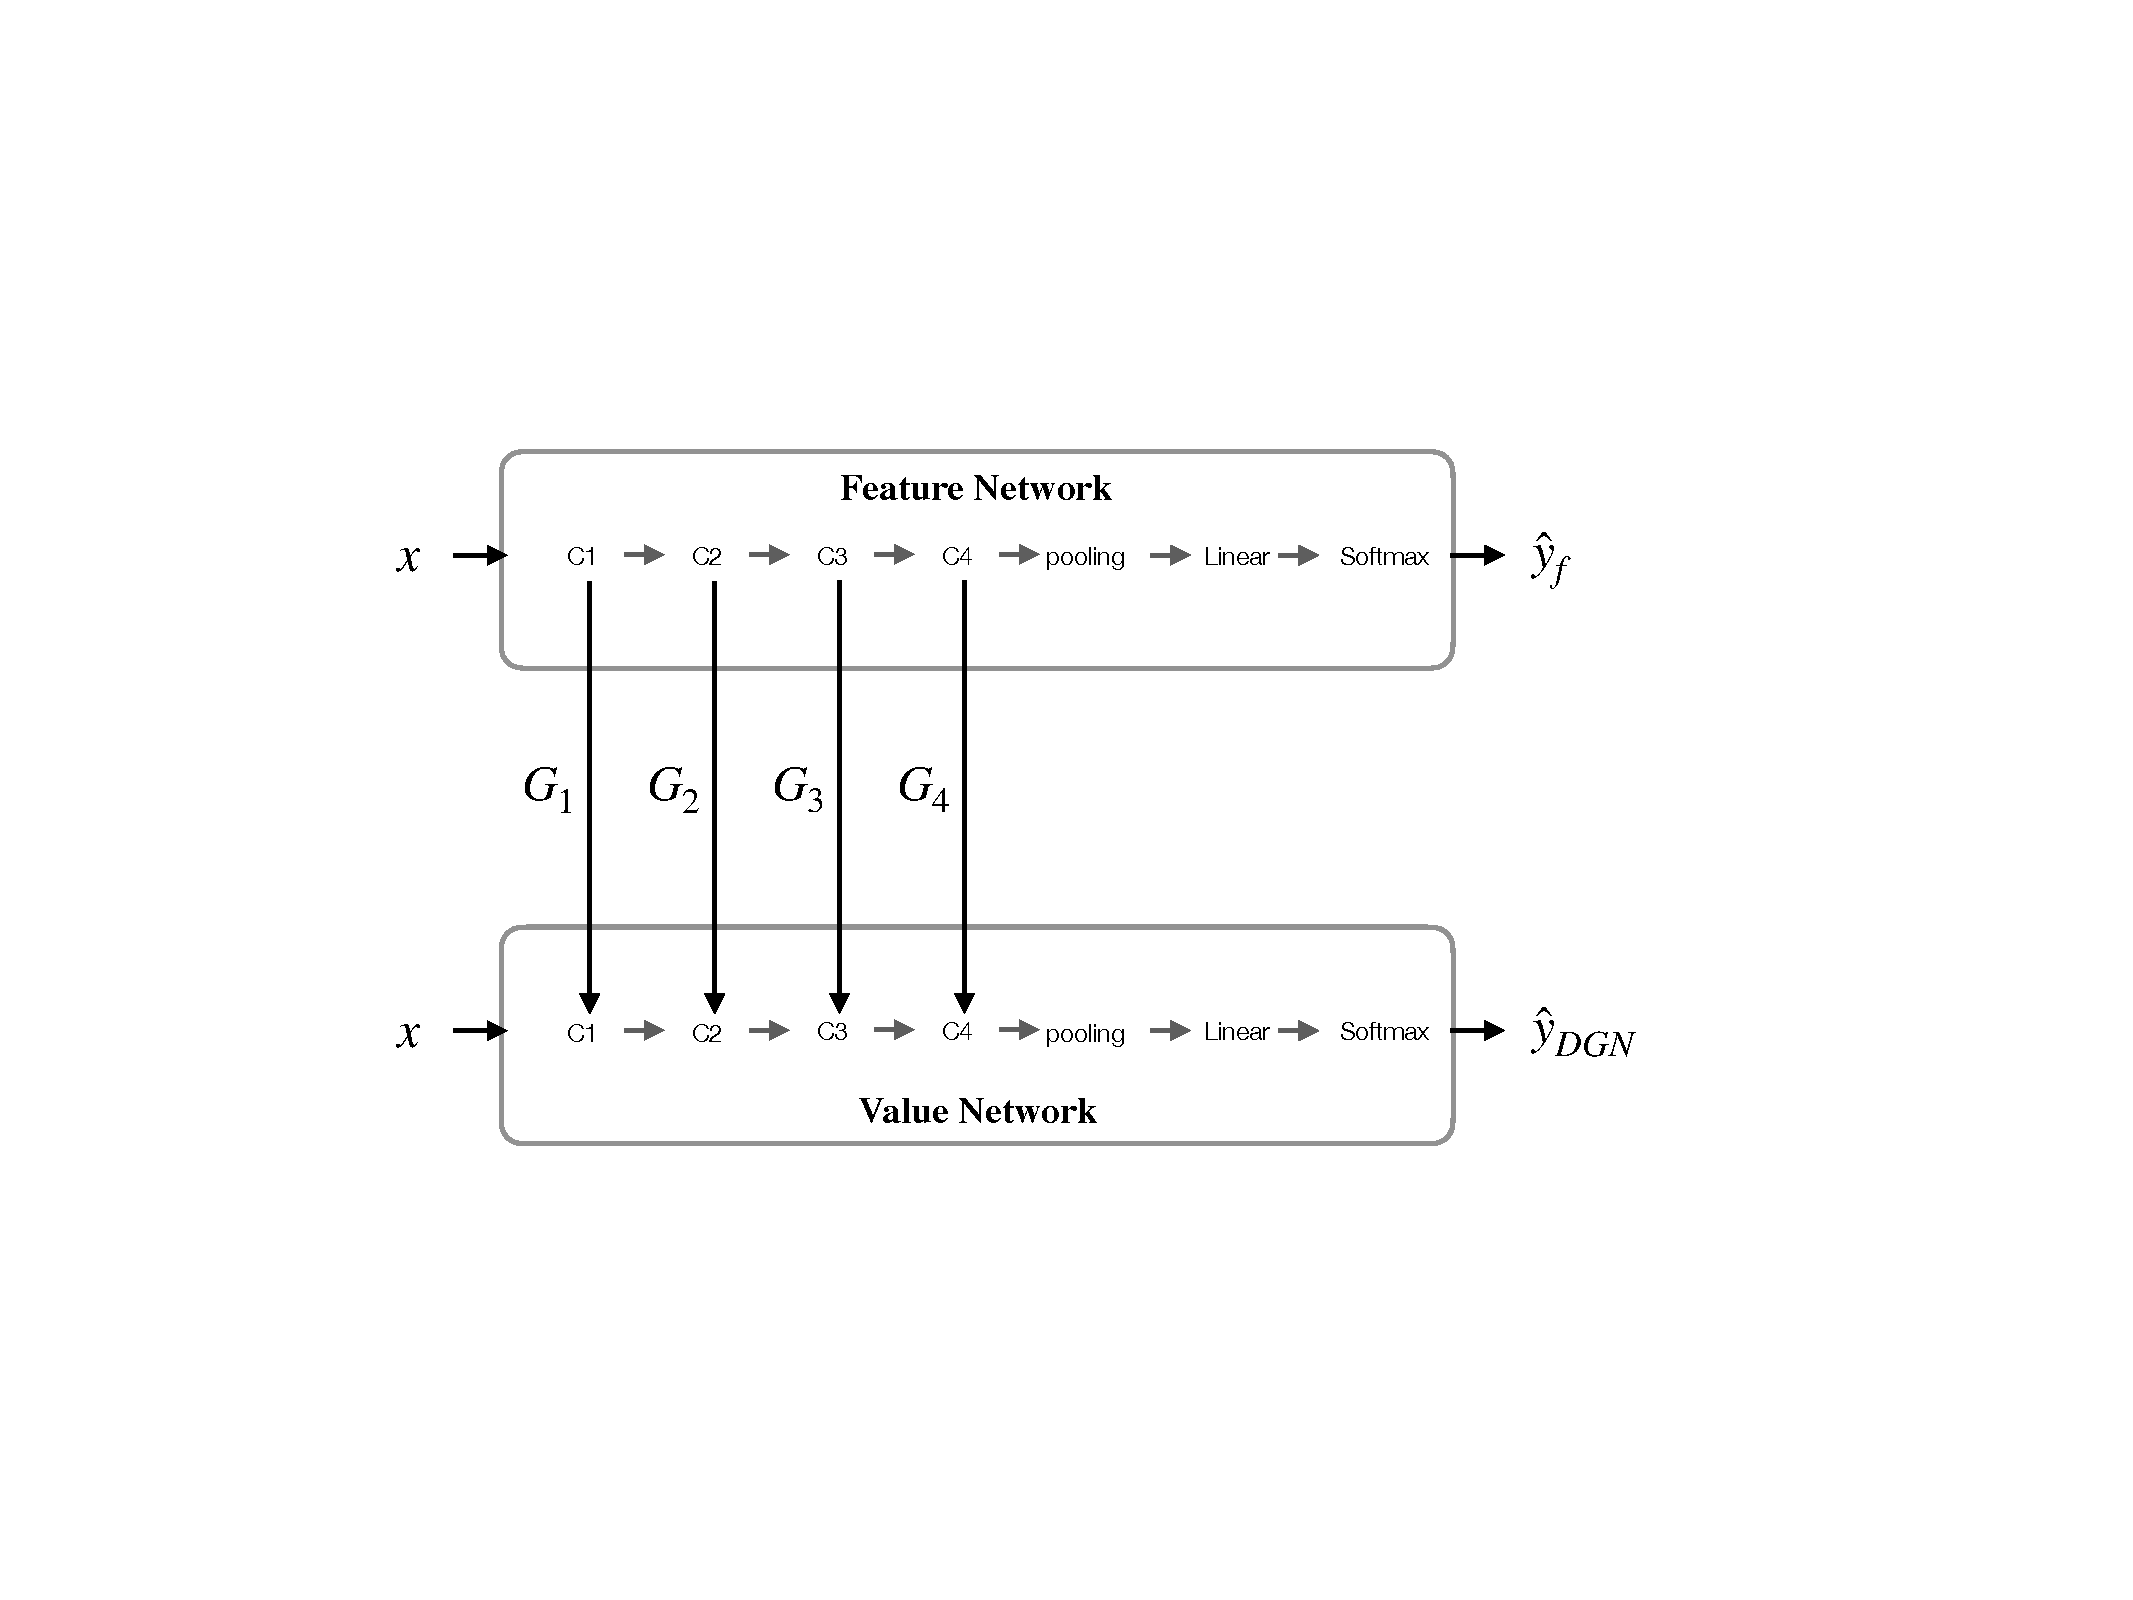
\includegraphics[scale=0.3]{figs/exp-prior.pdf}
}
\end{minipage}
\begin{minipage}{0.4\columnwidth}
\centering
\resizebox{\columnwidth}{!}{
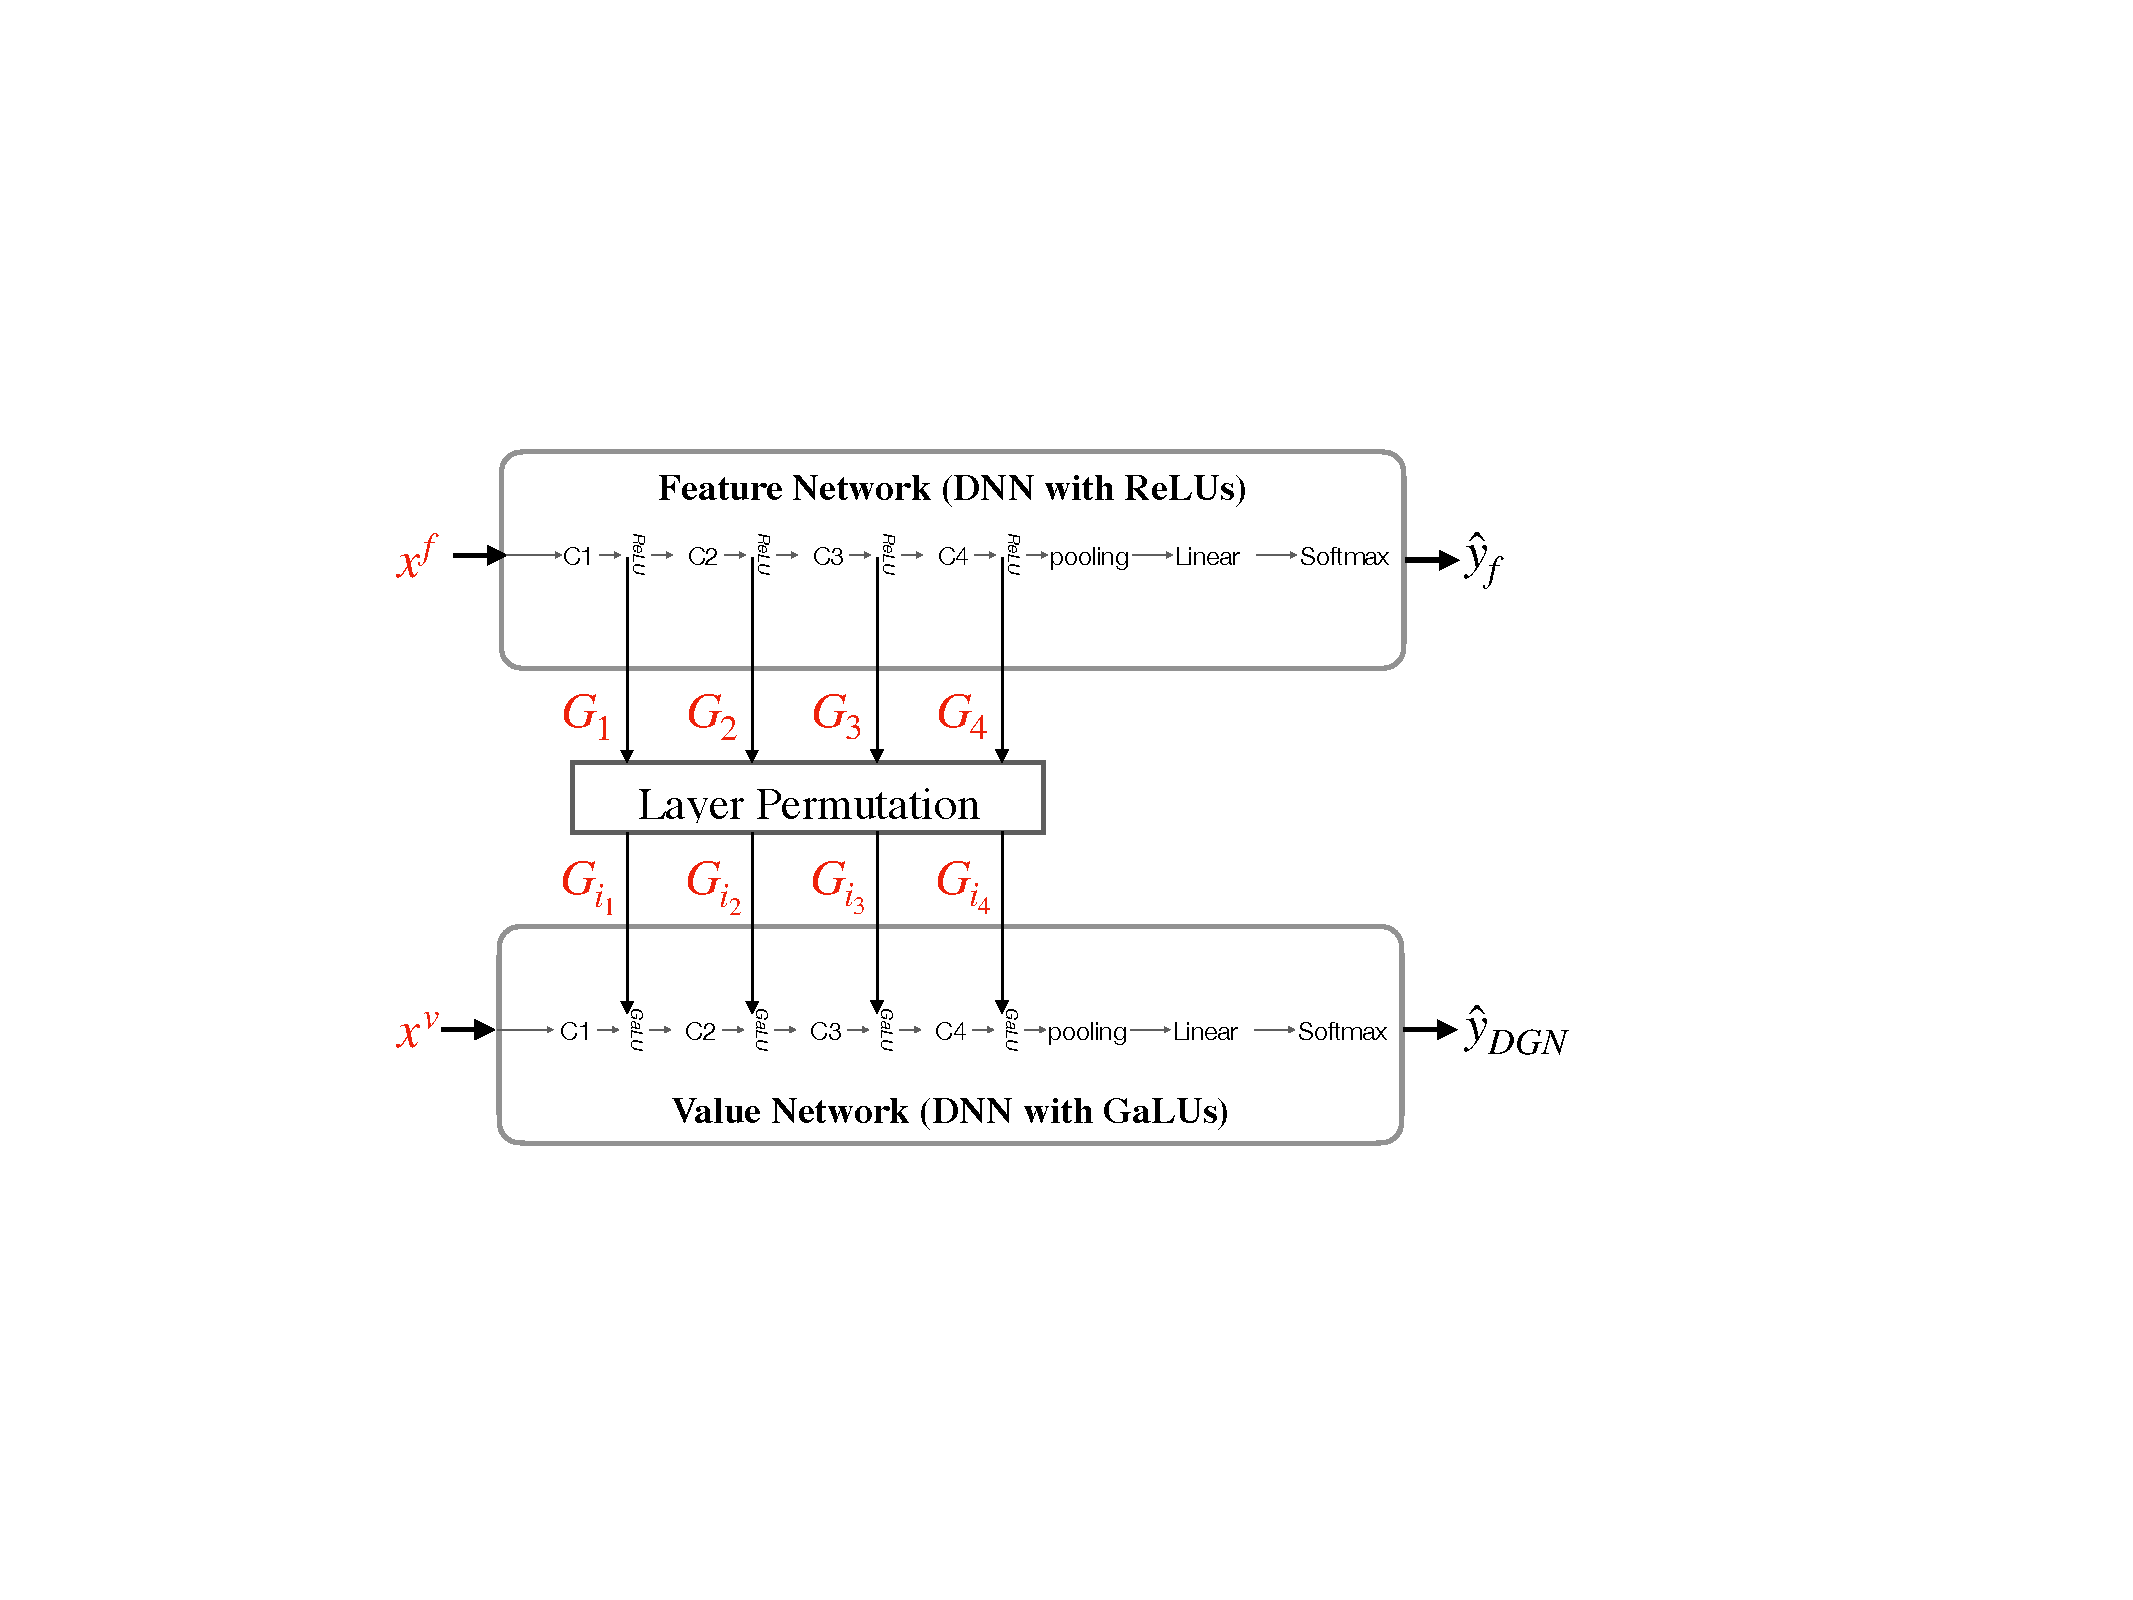
\includegraphics[scale=0.3]{figs/exp-new.pdf}
}
\end{minipage}
\caption{\small The prior setup in [\citenum{npk}] is shown in the left and the setup in this paper is shown in the right. Here $C1,\ldots,C4$ are convolutional layers with $128$ output filters, kernel size $3\times 3$ and stride $1\times 1$.}
\label{fig:dgn-prior-new}
\end{figure}
\begin{table}[t]
\centering
\begin{minipage}{0.95\columnwidth}
\begin{tabularx}{\columnwidth}{c *{5}{Y}}
\toprule
 Dataset& \multicolumn{2}{c}{Fixed Random}   &  \multicolumn{1}{c}{Decoupled} & \multicolumn{1}{c}{ Fixed } & \multicolumn{1}{c}{ReLU \tiny{(Feature Network)}}\\
& II & DI &Learning &Learnt &\\\hline\arrayrulecolor{white}\midrule
MNIST[\citenum{mnist}]& 94.1{\tiny{$\pm$0.3}}  &94.1\tiny{$\pm$0.3}  &98.1\tiny{$\pm$0.1} &98.6\tiny{$\pm$0.1} &98.5{\tiny{$\pm$0.1}}\\\hline
CIFAR-10[\citenum{cifar}]& 67.5\tiny{$\pm$0.7} &67.6\tiny{$\pm$0.7}   &77.6\tiny{$\pm$0.6} &79.4\tiny{$\pm$0.3} &80.4\tiny{$\pm$0.3}\\\hline
\arrayrulecolor{black}\bottomrule
\end{tabularx}
\end{minipage}
\caption{\small Shows the $\%$ test accuracy of various gates. The main result here is that the numbers in columns $1$ to $4$ are averaged over $48$ models (1 run per model, best performance in each run) and performance is robust to layer permutations and $x^{\text{v}}=\mathbf{1}$ input. For ReLU the average is over $5$ independent runs. Optimiser: Adam (3e-4). }
\label{tb:regimes}
\end{table}

\textbf{Note on prior results.} The following two observations were made in prior work [\citenum{npk}]: (i) by using the gates and training the NPV from scratch we can recover the performance (see ReLU vs Fixed Learnt in \Cref{tb:regimes}), and (ii) the performance of  Convolutional NTK ($77.43\%$)[\citenum{arora2019exact}] is between that of finite width network with random gates  ($67.5\%$) and learnt gates give ($79.4\%$), i.e., learning in the gates explains the difference between finite width DNNs and infinite width NTK.

\textbf{For `all-ones'} input to value network, in \Cref{th:main}, only $\ip{x,x'}=\din$, and $\Pi_{l=1}^{d-1}\frac{\ip{G_l(x),G_l(x')}}w$ is still unchanged. Similar explanations holds for \Cref{th:mainconv,th:mainres}.

\textbf{Robustness of Gates.} Entries in columns $1$ to $4$ in \Cref{tb:regimes} are  averaged over $48$ different models which included  permuting the layers and providing $\mathbf{1}$ as input. Our main result is that the information in the gates is robust over these $48$ models -- these justify the insights from \Cref{th:main} that as long as correlation in the gates is not destroyed the performance does not degrade. We also went one step further with respect to destroying the structure by considering arbitrary rotations. Here, we first tile the gates of the various filters (as a tensor) in the reverse order starting from layer $4$ to layer $1$ and then rotate arbitrarily in each of the three dimension for five times as shown in left of \Cref{fig:visual-permute} (i.e, two image dimensions and one filter dimension). For each rotation in the filter dimension we choose a random integer belonging to  $[0,512)$ and for each of the rotation in the image dimensions we choose a uniform random integer belonging to $[0,32)$. We did $10$ independent runs of the `fixed learnt' gates and `decoupled learning' of gates and observed the test performance to be $79.4${\tiny$\pm$0.2} and $79.0${\tiny$\pm$0.5} respectively (which are similar to the numbers shown in \Cref{tb:regimes}).

\begin{figure}[h]
\begin{minipage}{0.3\columnwidth}
\resizebox{\columnwidth}{!}{
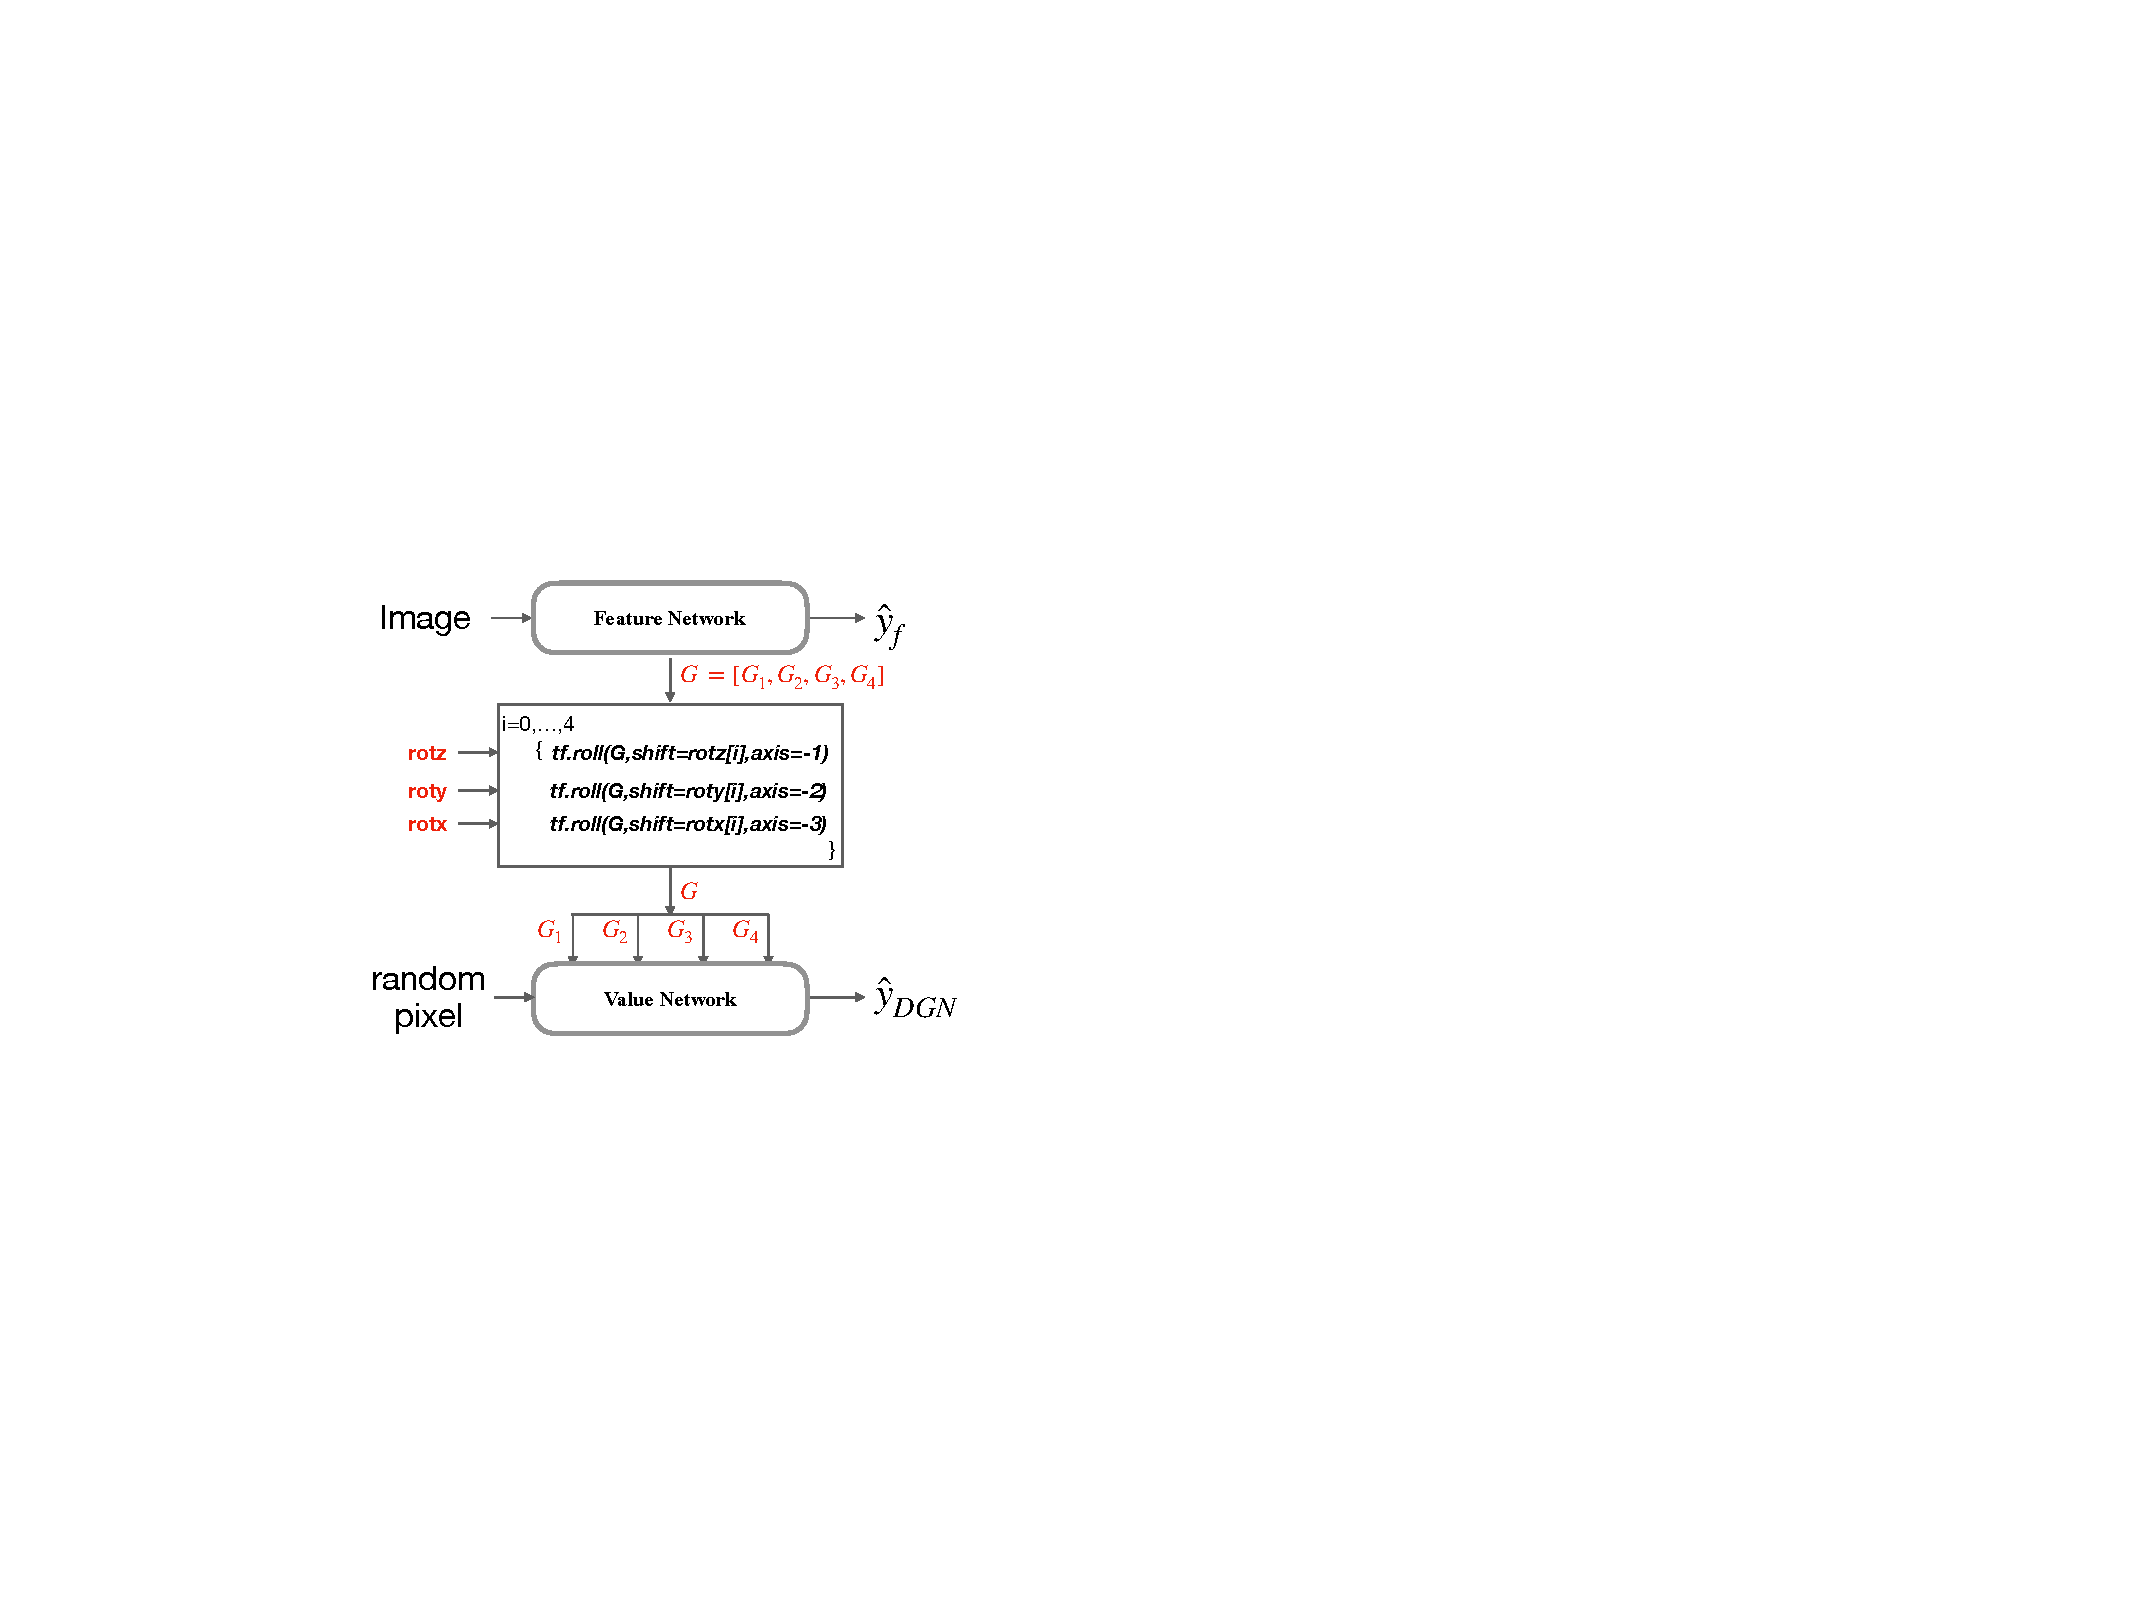
\includegraphics[scale=0.25]{figs/arbitrary_shift.pdf}
}
\end{minipage}
\begin{minipage}{0.68\columnwidth}
\resizebox{\columnwidth}{!}{
\begin{tabular}{cccccccccc}
&\Huge{Input}& \Huge{Layer 1, Filter 1}& \Huge{Layer 1, Filter 2}& \Huge{Layer 2, Filter 1}& \Huge{Layer 2, Filter 2}& \Huge{Layer 3, Filter 1}& \Huge{Layer 3, Filter 2}& \Huge{Layer 4, Filter 1}& \Huge{Layer 4, Filter 2}\\
\Huge{Feature Network}&\includegraphics{visual-iclr/images/horse.png}&
\includegraphics{images_neurips_2021/feature_network/layer_1_0.png}&
\includegraphics{images_neurips_2021/feature_network/layer_1_1.png}&
\includegraphics{images_neurips_2021/feature_network/layer_2_0.png}&
\includegraphics{images_neurips_2021/feature_network/layer_2_1.png}&
\includegraphics{images_neurips_2021/feature_network/layer_3_0.png}&
\includegraphics{images_neurips_2021/feature_network/layer_3_1.png}&
\includegraphics{images_neurips_2021/feature_network/layer_4_0.png}&
\includegraphics{images_neurips_2021/feature_network/layer_4_1.png}\\
\Huge{Value Network}&\includegraphics{images_neurips_2021/allones.png}&
\includegraphics{images_neurips_2021/value_network//layer_1_0.png}&
\includegraphics{images_neurips_2021/value_network//layer_1_1.png}&
\includegraphics{images_neurips_2021/value_network//layer_2_0.png}&
\includegraphics{images_neurips_2021/value_network//layer_2_1.png}&
\includegraphics{images_neurips_2021/value_network//layer_3_0.png}&
\includegraphics{images_neurips_2021/value_network//layer_3_1.png}&
\includegraphics{images_neurips_2021/value_network//layer_4_0.png}&
\includegraphics{images_neurips_2021/value_network//layer_4_1.png}
\end{tabular}
}

\end{minipage}
\caption{Top (Standard CNN): First image on the left is the input image and the next $8$ images are outputs of $2$ filters in each of the $4$ layers. Bottom (DGN with gates of the top model applied in reverse order): First image on the left is the input to the value network and the next $8$ images are outputs of $2$ filters in each of the $4$ layers. Both models achieve a test accuracy of about $80\%$.}
\label{fig:visual-permute}
\end{figure}

\textbf{Primal vs Dual View of features.} The standard (primal) view is that the input is processed layer-by-layer and the hidden features are in the layer outputs. 
%The dual view is that the features are encoded in the gates (analytically speaking the NPF/NPK). While both are mathematically equivalent, we believe that the dual view paints more accurate picture. 
Our experiments challenge the primal view, because, 
we do not provide the image as input but only $\mathbf{1}$ (`all-ones') as input to the value network, and we have destroyed the layer-by-layer structure of the gates before applying them as masks in the value network as well (also, the `fixed learnt' gates do not change during training). As a result, there is a huge `visual' difference between the hidden layer outputs of the feature network and that of the value network (see right of \Cref{fig:visual-permute}).  One could still insist that DNNs are so powerful that they are recovering the features layer-by-layer. Or alternatively, one can appeal to the dual view to conclude that since neither `all-ones' input nor the arbitrary rotation of the gates affect the correlation of gates (\Cref{th:main}), the performance does not degrade. While the gates are generated layer-by-layer in the feature network, when applied as masks, the function of the gates is to select and train the sub-networks corresponding to each example (viewpoint trivially following from \Cref{prop:npf-npv}) .
\begin{comment}
\textbf{Primal vs Dual View of features.} The standard (primal) view is that the input is processed layer-by-layer and the hidden features are in the layer outputs. To challenge this view, 
%The dual view is that the features are encoded in the gates (analytically speaking the NPF/NPK). While both are mathematically equivalent, we believe that the dual view paints more accurate picture. Our experiments challenge the primal view. 
we do not provide the image as input but only $\mathbf{1}$ (`all-ones') as input to the value network. Now, it could be argued that the value network gets the information about the via its gating masks. To counter this argument, we have destroyed the layer-by-layer structure of the gates before applying them as masks in the value network as well. As a result, there is a huge `visual' difference between the hidden layer outputs of the feature network and that of the value network (see right of \Cref{fig:visual-permute}).  One could still insist that DNNs are so powerful that they are recovering the features layer-by-layer. Or alternatively, one can appeal to the dual view to conclude that since neither `all-ones' input nor the arbitrary rotation of the gates affect the correlation of gates (\Cref{th:main}), the performance does not degrade. While the gates are generated layer-by-layer in the feature network, when applied as masks, the function of the gates is to learn and train the paths and sub-networks (viewpoint trivially following from \Cref{prop:npf-npv}) .
\end{comment}

\textbf{Gate learning need not be layer-by-layer.} In `decoupled learning' (\Cref{tb:regimes}), while the gates are generated layer-by-layer in the feature network, after arbitrary rotations they end in a different location in the value network during training, i.e., the gates can be arbitrarily placed while learning.
\subsection{Upstream training with random labels and downstream with true labels affects the gates}\label{sec:exp2}
\textbf{Q1 (open question [\citenum{randlabel}]).} {When trained with random labels upstream followed by true labels downstream, the test performance of a DNN with ReLUs degrades, Why?}

\textbf{Setup to answer Q1.} We hypothesise that the answer to the above question lies in the gates. To test our hypothesis, we train in two phases (i) Phase I: upstream training with label noise levels $\gamma=0, 25\%, 50\%, 75\%$ and (ii) Phase II: downstream training with true labels. For $\gamma=0$ there is no Phase II because Phase I is already with true labels. We then measure the information stored in the gates at the end of each of the two phases. To this end, we consider the DGN setup in \Cref{fig:dgn-prior-new} (left), and train the feature network (which is a DNN with ReLUs) with $\hat{y}_{\text{f}}$ as output node. In Phase I, we train the feature network for different values of label noise $\gamma=0, 25\%, 50\%, 75\%$, which gives us models $M1(\gamma)$ (see \Cref{fig:rand-label-setup}). To measure the information in the gates learnt at the end of Phase I, we keep these gates fixed and train the value network with true labels -- this gives us models $M2(\gamma)$ (see \Cref{fig:rand-label-setup}). In Phase II, we start with models $M1(\gamma)$ (i.e., obtained at end of Phase I), and perform downstream training with true labels to obtain models $M4(\gamma)$.  To measure the information in the gates learnt at the end of Phase II, we keep these gates fixed and train the value network with true labels -- this gives us models $M5(\gamma)$ (see \Cref{fig:rand-label-setup}).

\begin{figure}[t]
\centering
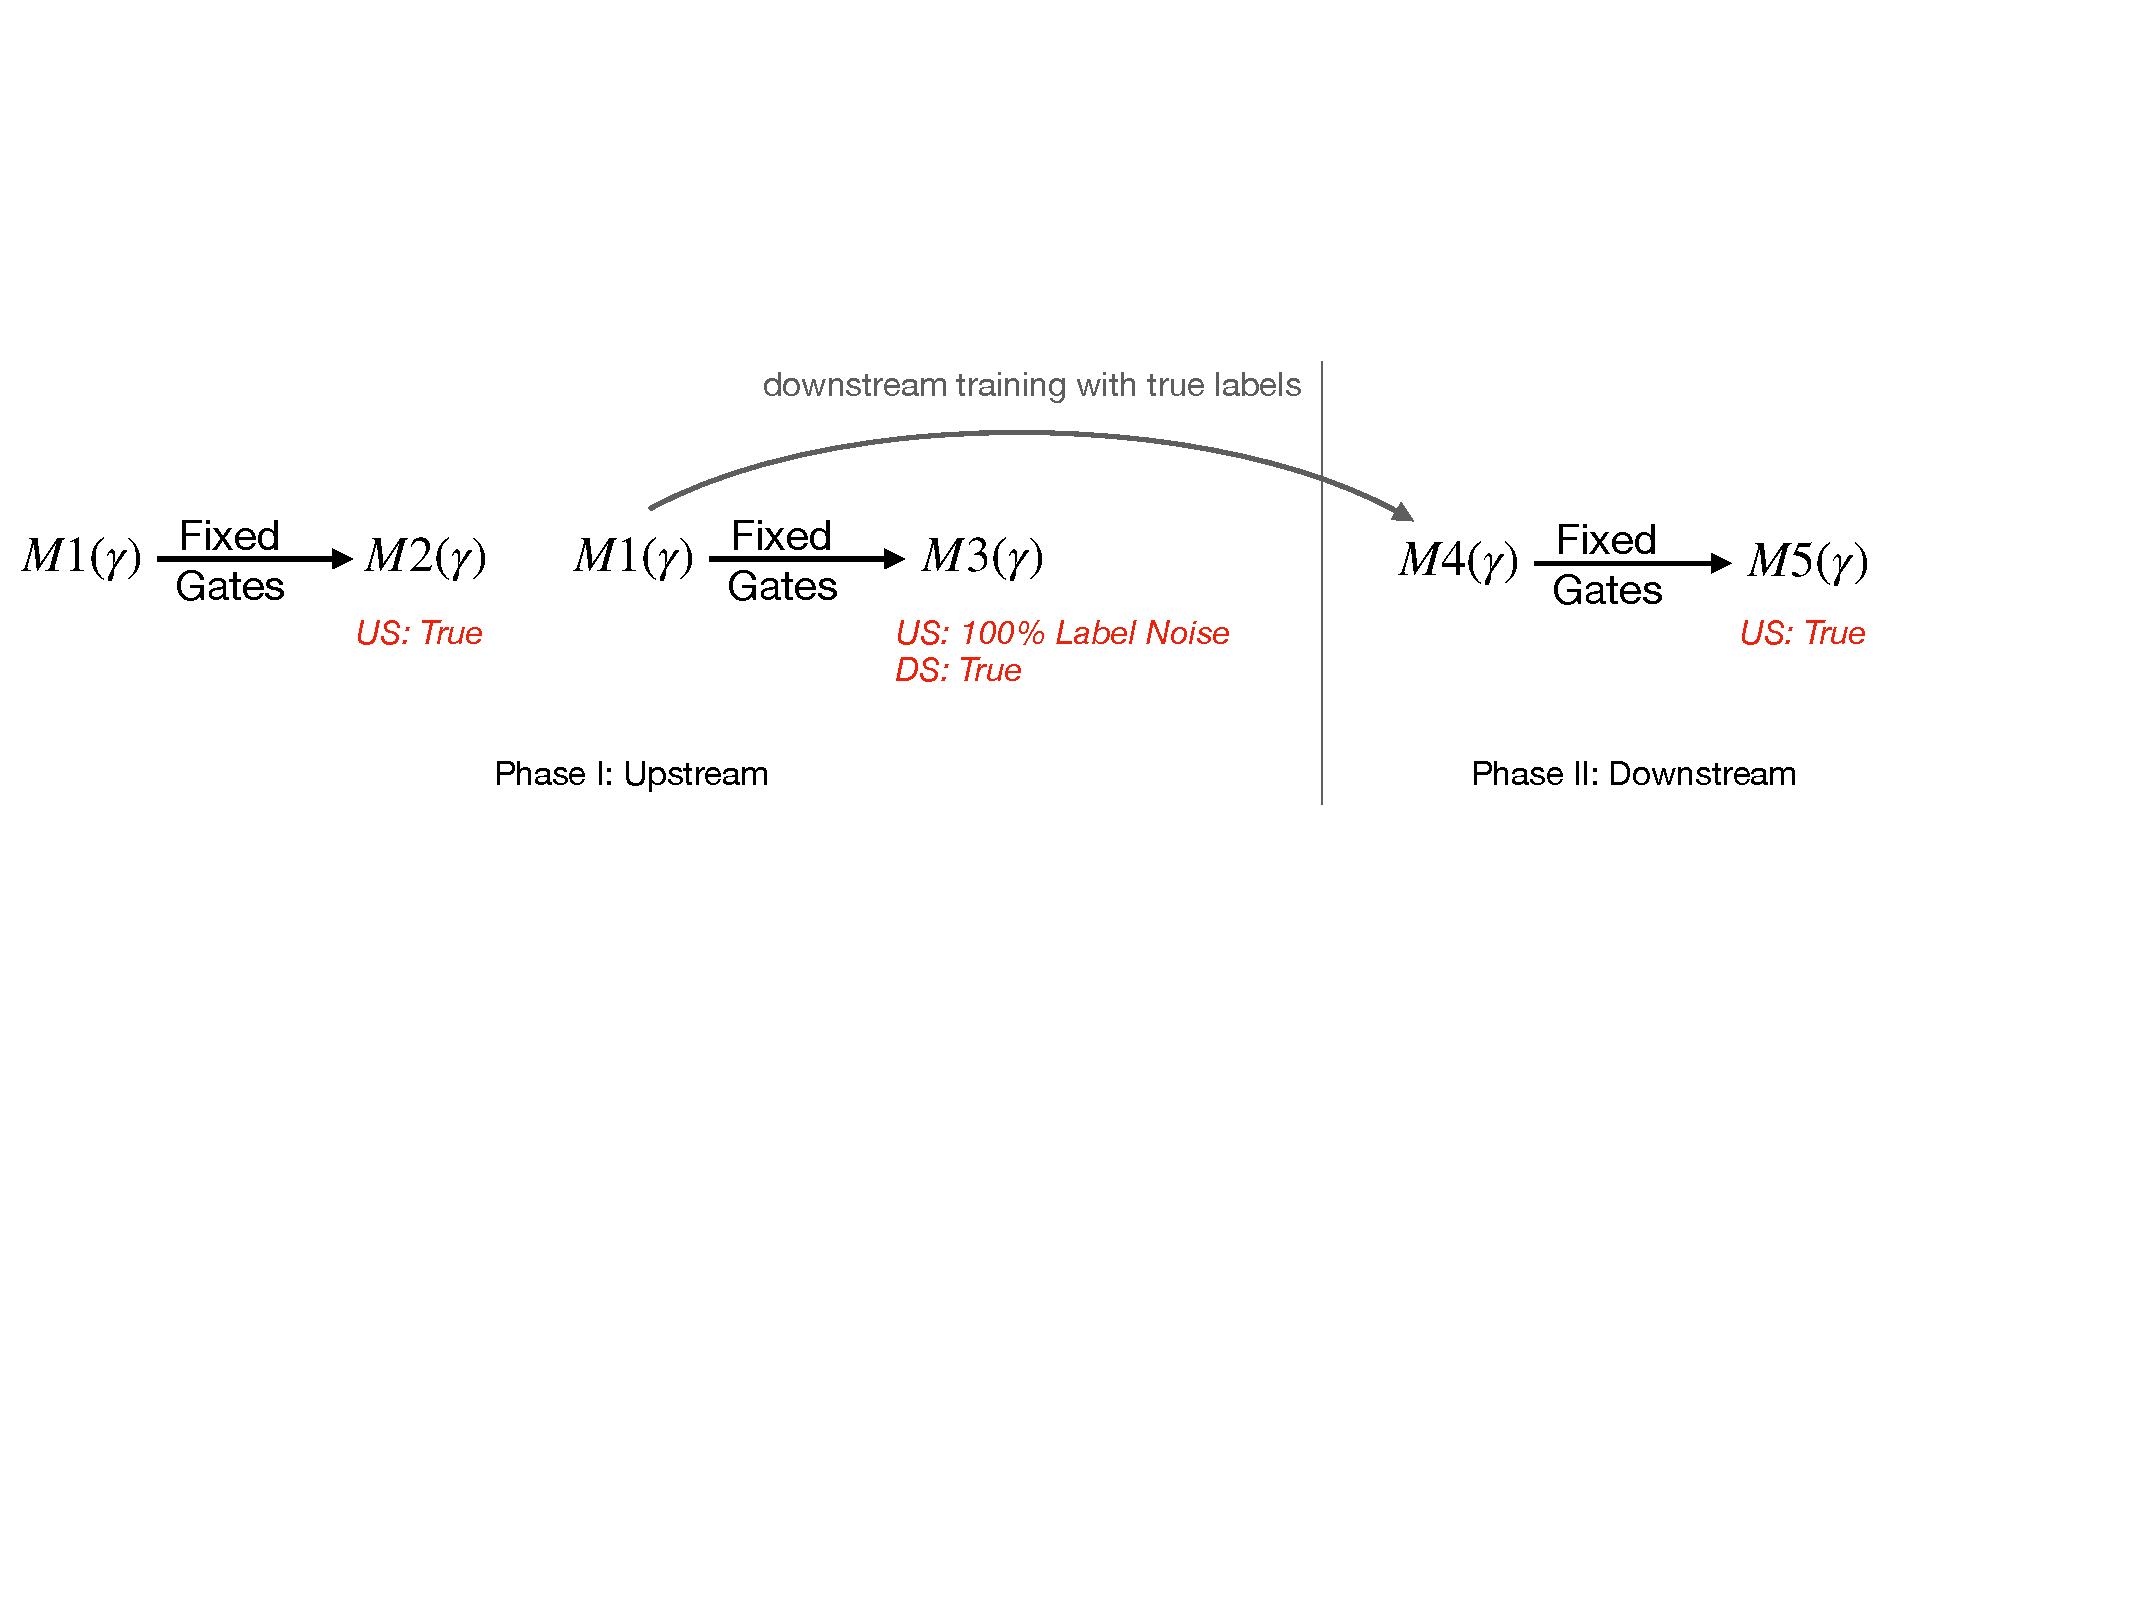
\includegraphics[scale=0.25]{figs/rand-label-big.pdf}
\caption{\small Shows various models trained in Experiment 2. Here, US and DS stand for upstream and down stream respectively. True for training with true labels. Here models $M1$ and $M4$ are feature networks (DNNs with ReLUs), and $M2, M3$ and $M5$ are value networks which use the fixed gates from the feature networks. Models are parameterised by $(\gamma)$ which is the label noise level.}
\label{fig:rand-label-setup}
\end{figure}


\textbf{Q2 (new question).} {When trained with random labels upstream followed by true labels downstream, \emph{if the gates are fixed throughout and only the weights are trained}, does the test performance degrade?}

\textbf{Setup to answer Q2.} Here, we pick up the models trained at the end of Phase I, use them as feature networks and fix the gates. We then train the value network, first upstream with with $100\%$ random labels, and then downstream with $100\%$ true labels--this gives us models $M3(\gamma)$.

The results of the experiments with random labels shown in \Cref{tb:rand-label} (plots are in the Appendix).

\textbf{Answer to Q2.} \emph{When the gates are fixed test performance is robust to upstream training with random labels.} In  \Cref{tb:rand-label}, look at the performance of $M3(\gamma=0)$ and compare it with performance of  $M4(\gamma), \gamma=25,50,75$. When the gates are fixed, i.e., in $M3(0)$ (note: this is a value network), the upstream training with even $100\%$ label noise does not hurt the test performance so much ($81.2-79.3 <2\%$) in comparison to the cases when the gates are allowed to change, i.e., $M4(\gamma)$ (note: these are feature networks), the test performance degrades (from $81.2$) to $76.9$ ( $ 4.3\%$ for $\gamma=25$), $73.6$ ( $7.6\%$ for $\gamma=50$) and  $68.1$ ($13.1\%$ for $\gamma=75$) for even less than $100\%$ label noise.
%\begin{comment}
\begin{table}[t]
\centering
\resizebox{0.8\columnwidth}{!}{
\begin{tabularx}{\columnwidth}{c *{6}{Y}}
\toprule
 & \multicolumn{4}{c}{Phase I: Upstream}  
 & \multicolumn{2}{c}{Phase II: Downstream}\\
\cmidrule(lr){2-5} \cmidrule(l){6-7}
&  \multicolumn{2}{c}{ReLU}  &\multicolumn{2}{c}{Fixed Gates} & ReLU & {Fixed Gates}\\
\cmidrule(lr){2-3} \cmidrule(lr){4-5}\cmidrule(lr){6-7}
$\gamma$& Best & End & True& US\&DS & True & True\\\hline\arrayrulecolor{white}\midrule
0 &{\bf{81.2}}{\tiny $\pm$ 0.3} & 80.0{\tiny $\pm$ 0.4} &{\bf{80.3}}{\tiny $\pm$ 0.2} & {\bf{79.3}}{\tiny $\pm$ 0.4} &-&- \\\hline
{25}&76.1{\tiny $\pm$ 0.6} & 63.1{\tiny $\pm$ 0.7}& 74.7{\tiny $\pm$ 0.5}& 72.3{\tiny $\pm$ 0.2}&76.9{\tiny $\pm$ 0.1}&76.9{\tiny $\pm$ 0.4}\\\hline
{50}&70.9{\tiny $\pm$ 0.8} & 41.5{\tiny $\pm$ 1.1}& 69.9{\tiny $\pm$ 0.3} & 66.8{\tiny $\pm$ 0.1}&73.4{\tiny $\pm$ 0.3}&73.6{\tiny $\pm$ 0.4}\\\hline
{75}&56.9{\tiny $\pm$ 0.4} & 23.4{\tiny $\pm$ 0.4}& 63.9{\tiny $\pm$ 0.4} &60.0{\tiny $\pm$ 0.3}&68.1{\tiny $\pm$ 0.4}&67.7{\tiny $\pm$ 0.6}\\\hline
\arrayrulecolor{black}\bottomrule
Models & \multicolumn{2}{c}{M1($\gamma$)} & M2($\gamma$) & M3($\gamma$)& M4($\gamma$) & M5($\gamma$)\\\bottomrule
\end{tabularx}
}
\caption{\small Shows the $\%$ test accuracy (on test data with true labels) of the models in Experiment 2 on CIFAR-10. The numbers are averaged over $3$ runs (best accuracy is taken in each run except for column `End'). For column `End', in each run the average test accuracy over the last $10$ epochs are considered. Optimiser: Adam(3e-4).}
\label{tb:rand-label}
\end{table}
%\end{comment}
\begin{comment}
\begin{table}[t]
\begin{tabularx}{\columnwidth}{c *{6}{Y}}
\toprule
 & \multicolumn{2}{c}{Phase I} &  \multicolumn{2}{c}{Phase I End} &{Phase II}&  \multicolumn{1}{c}{Phase II End}\\
\cmidrule(lr){2-3} \cmidrule(lr){4-5} \cmidrule(l){6-6}\cmidrule(l){7-7}
&  \multicolumn{2}{c}{ReLU}  &\multicolumn{2}{c}{Fixed Gates} & ReLU &  \multicolumn{1}{c}{Fixed Gates }\\
\cmidrule(lr){2-3} \cmidrule(lr){4-5} \cmidrule(l){6-6}\cmidrule(l){7-7}
$\gamma$& Best & End & True& US/DS & True & True\\\hline\arrayrulecolor{white}\midrule
0 &{\bf{81.2}}{\tiny $\pm$ 0.3} & 80.0{\tiny $\pm$ 0.4} &{\bf{80.3}}{\tiny $\pm$ 0.2} & {\bf{79.3}}{\tiny $\pm$ 0.4} &-&- \\\hline\hline
{25}&76.1{\tiny $\pm$ 0.6} & 63.1{\tiny $\pm$ 0.7}& 74.7{\tiny $\pm$ 0.5}& 72.3{\tiny $\pm$ 0.2}&76.9{\tiny $\pm$ 0.1}&76.9{\tiny $\pm$ 0.4}\\\hline\hline
{50}&70.9{\tiny $\pm$ 0.8} & 41.5{\tiny $\pm$ 1.1}& 69.9{\tiny $\pm$ 0.3} & 66.8{\tiny $\pm$ 0.1}&73.4{\tiny $\pm$ 0.3}&73.6{\tiny $\pm$ 0.4}\\\hline\hline
{75}&56.9{\tiny $\pm$ 0.4} & 23.4{\tiny $\pm$ 0.4}& 63.9{\tiny $\pm$ 0.4} &60.0{\tiny $\pm$ 0.3}&68.1{\tiny $\pm$ 0.4}&67.7{\tiny $\pm$ 0.6}\\\hline
\arrayrulecolor{black}\bottomrule
Models & \multicolumn{2}{c}{$M1(\gamma)$} & $M2(\gamma)$ & $M3(\gamma)$& $M4(\gamma)$ & $M5(\gamma)$\\\bottomrule
\end{tabularx}
\caption{\small Shows the $\%$ test accuracy (on test data with true labels) of the various models in Experiment 2 on CIFAR-10. The numbers are averaged over $3$ runs (best accuracy is taken in each run except for column `End'). For column `End', in each run the average test accuracy over the last $10$ epochs are considered. Optimiser: Adam(3e-4). The plots are in the Appendix.}
\label{tb:rand-label}
\end{table}
\end{comment}

\textbf{Answer to Q1.} Recall from \Cref{prop:npf-npv} that in a DNN with ReLUs (which is the feature network), $\hat{y}_{\Tf}(x)=\ip{\phi_{x,\Tf},v_{\Tf}}$, and when training, both $\phi_{x,\Tf}$ and $v_{\Tf}$ are learnt. We now examine how random labels affect $\phi_{x,\Tf}$ and $v_{\Tf}$. During upstream training, the test performance initially improves, reaches a `Best' and then degrades (see `Best' and `End' in \Cref{tb:rand-label}). Now, if we use the NPFs $\phi_{x,\Tf}$ (i.e., gates) at the end of Phase I and train the NPV ($v_{\Tv}$) separately in the value network to obtain $M2(\gamma)$ we see that $M2(\gamma)$ is better than the `Best' of $M1(\gamma)$. This implies degradation post the `Best' value mostly affects only the NPV ($v_{\Tf}$) and not the NPFs. Yet, the NPFs $\phi_{x,\Tf}$ at end of Phase I, i.e., $M2(\gamma), \gamma=25,50,75$ are worser than $M2(0)$. Now, even when we perform downstream training with true labels in Phase II, the recovery is not full (i.e., $M4(\gamma)$ are not close to $M1(0)=81.2$). After both Phases I and II, both $\phi_{x,\Tf}$ and $v_{\Tf}$ have gone through upstream as well as downstream training, and the lack of recovery could be due to either $\phi_{x,\Tf}$  or $v_{\Tf}$. In order to separate this we take only the NPFs $\phi_{x,\Tf}$ (i.e., gates at end of Phase II) and retrain the NPV ($v_{\Tv }$) afresh with true labels in the value network to obtain $M5(\gamma)$. Now from the fact that $M5(\gamma) \approx M4(\gamma)$, we know that the NPFs $\phi_{x,\Tf}$ (i.e., the gates) are the real reason for the degradation. We can conclude that (i) \emph{the degradation in test performance is due to the gates (i.e., NPFs), and (ii) gates (i.e., NPFs) do resist such degradation (i.e., after the `Best' the NPFs do not degrade)}.

\begin{comment}
\begin{figure}[h]
\begin{minipage}{0.99\columnwidth}
\resizebox{\columnwidth}{!}{
\begin{tabular}{ccc}
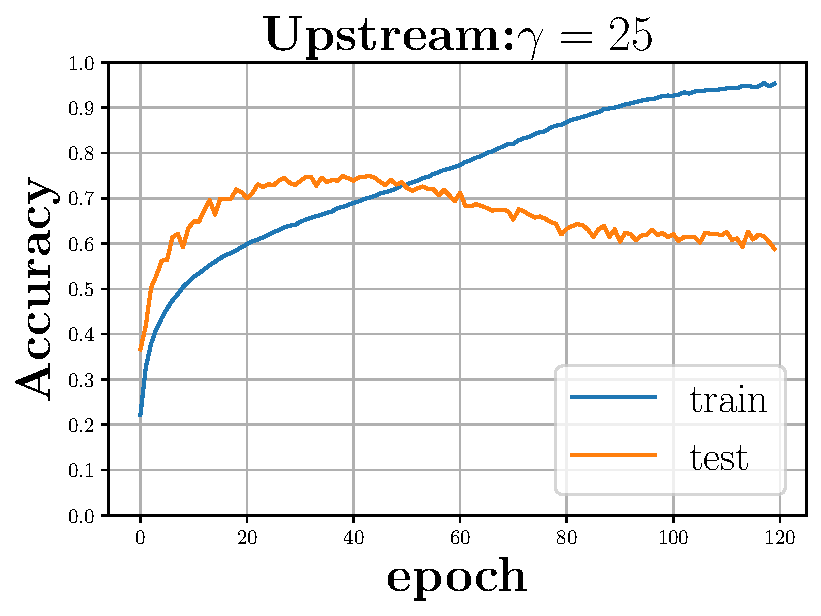
\includegraphics[scale=0.125]{figs/relu_25.pdf}&
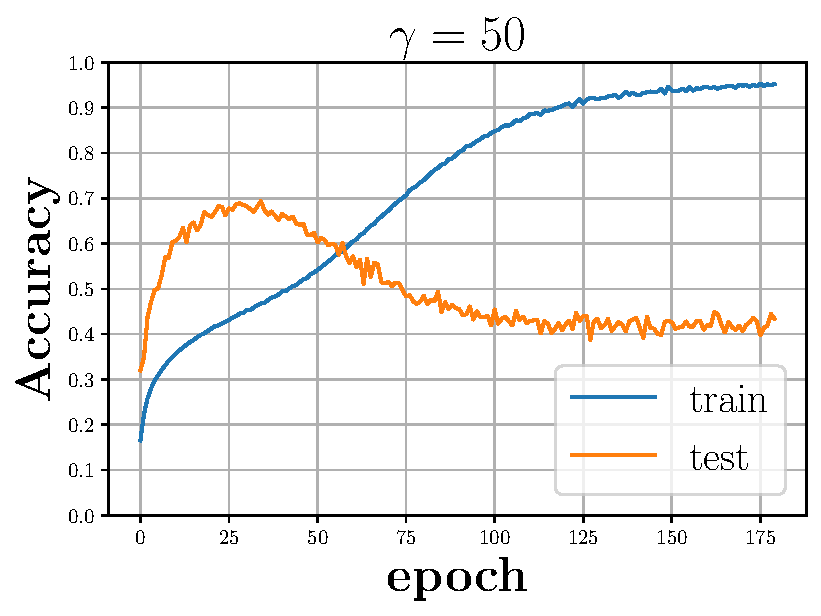
\includegraphics[scale=0.125]{figs/relu_50.pdf}&
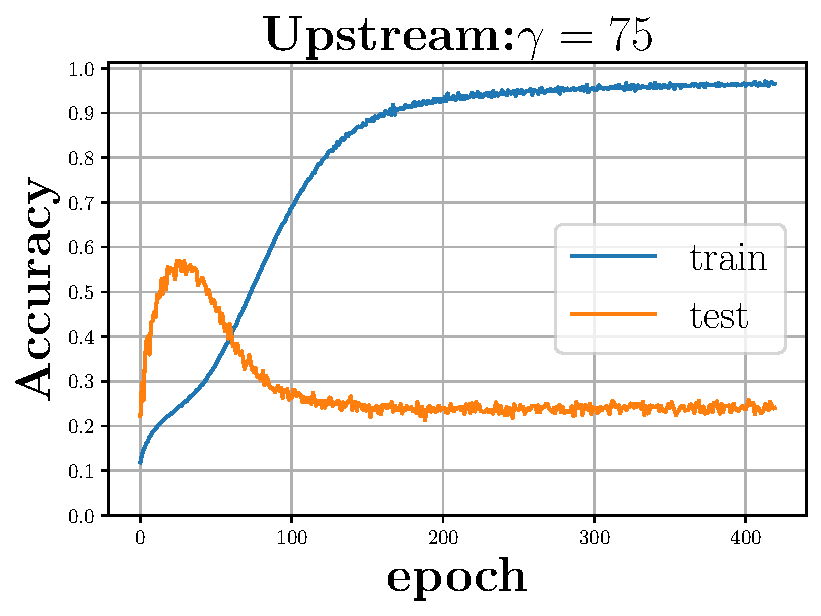
\includegraphics[scale=0.125]{figs/relu_75.pdf}
\\
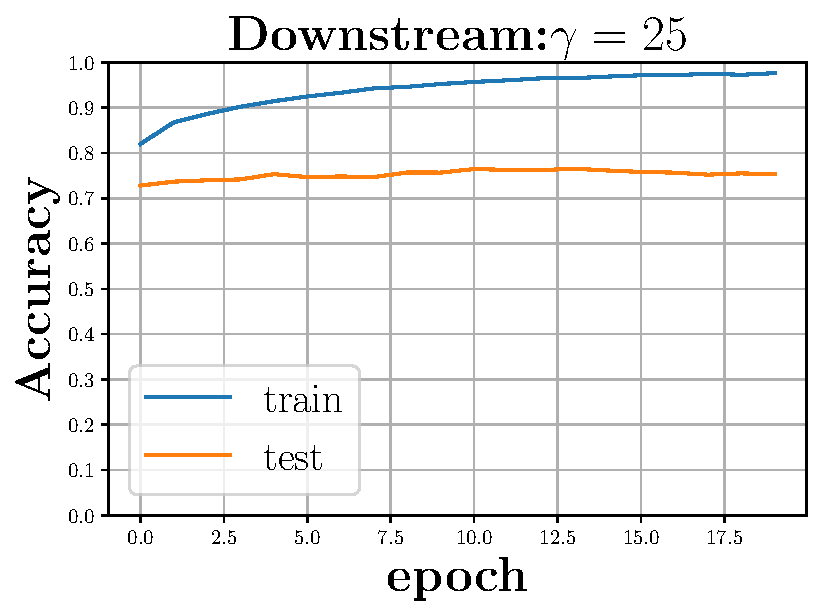
\includegraphics[scale=0.125]{figs/relu_25_good.pdf}&
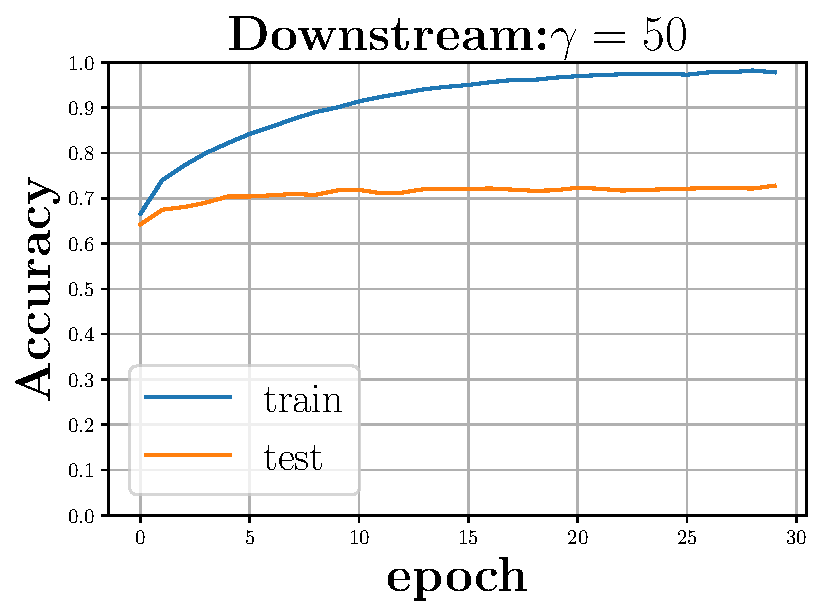
\includegraphics[scale=0.125]{figs/relu_50_good.pdf}&
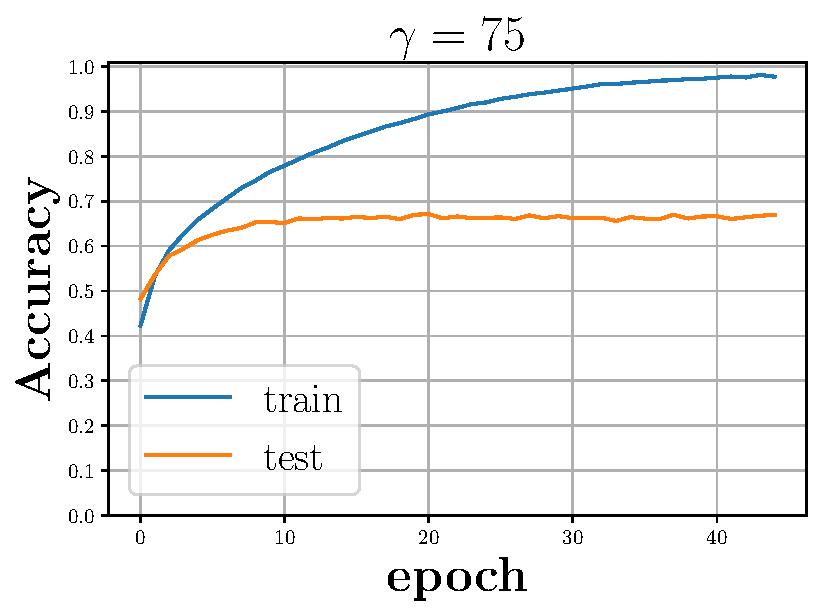
\includegraphics[scale=0.125]{figs/relu_75_good.pdf}\\
\end{tabular}
}
\end{minipage}
\caption{Shows the upstream training with random labels followed downstream training with true labels. The first epochs of bottom plots is same as the epoch follows the last epoch in the top plots.}
\label{fig:rand-label}

\end{figure}
\end{comment}

\begin{comment}
\begin{figure}[h]
%\begin{comment}
\begin{minipage}{0.4\columnwidth}
\resizebox{\columnwidth}{!}{
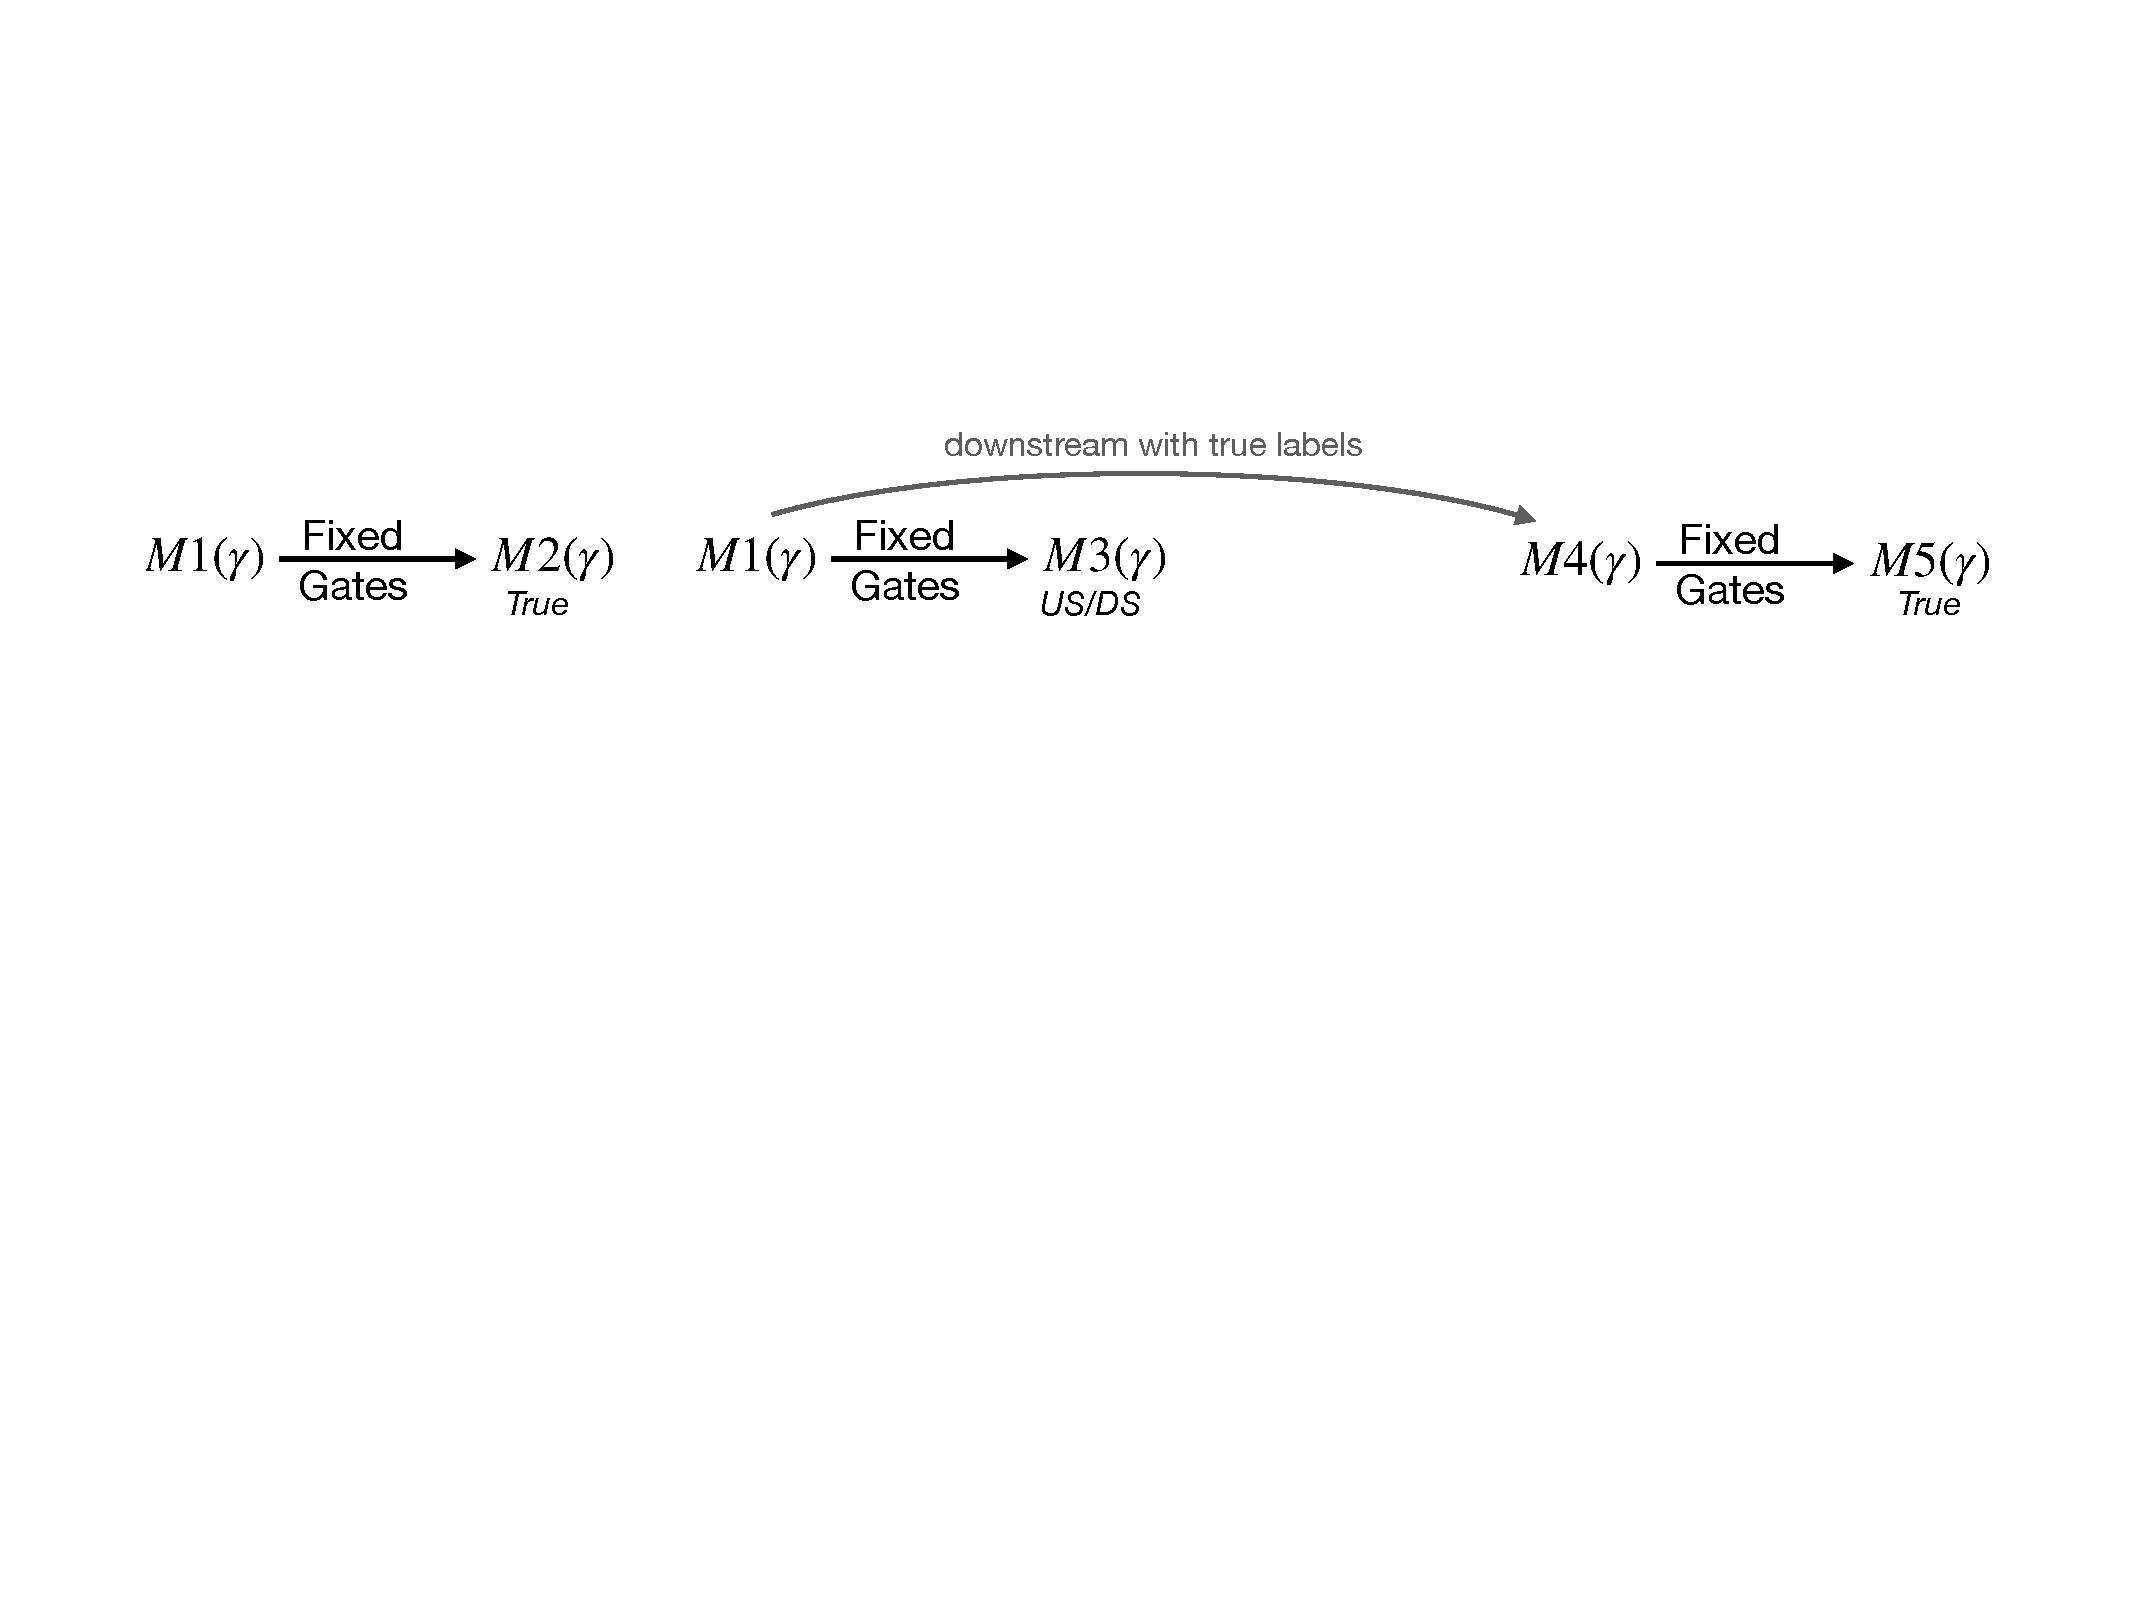
\includegraphics[scale=0.35]{figs/rand-label.pdf}
}
\end{minipage}
%\end{comment}
\begin{minipage}{0.99\columnwidth}
\resizebox{\columnwidth}{!}{
\begin{tabular}{cccccc}
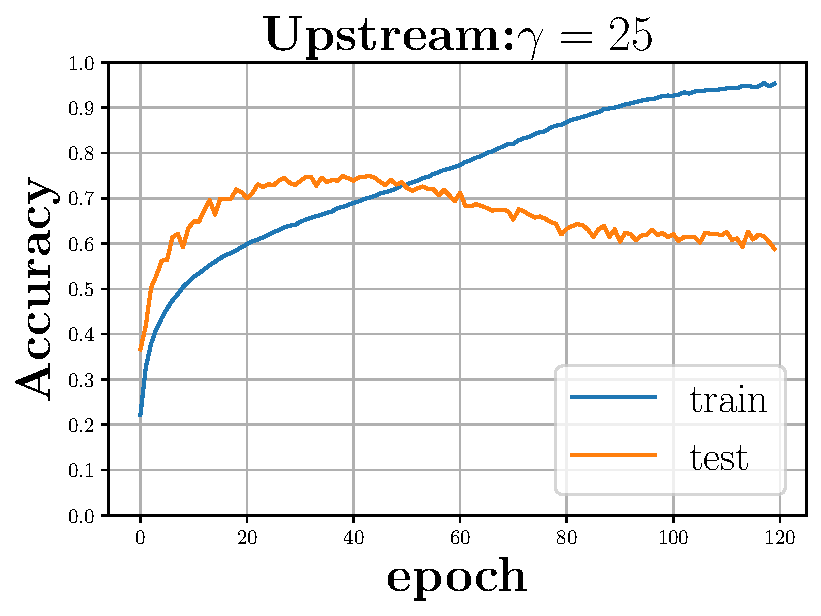
\includegraphics[scale=0.125]{figs/relu_25.pdf}&
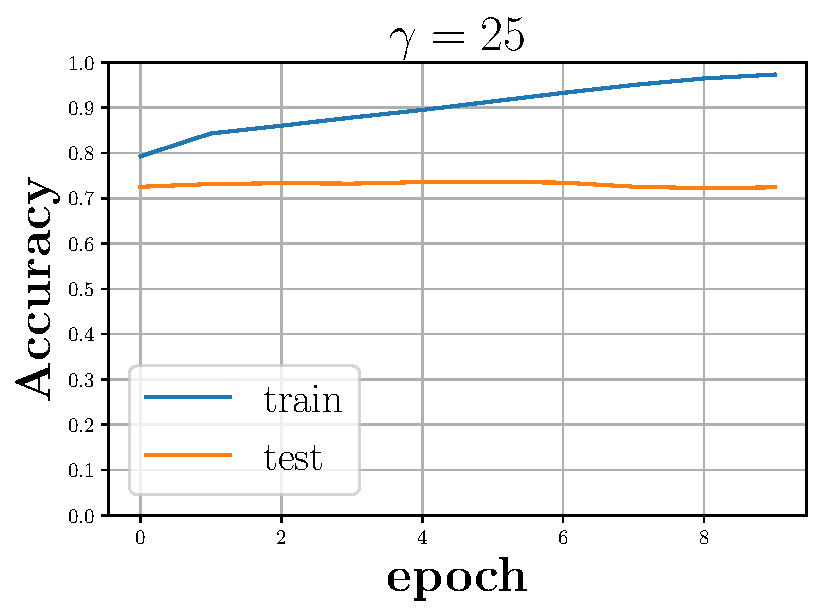
\includegraphics[scale=0.125]{figs/galu_25_good.pdf}&
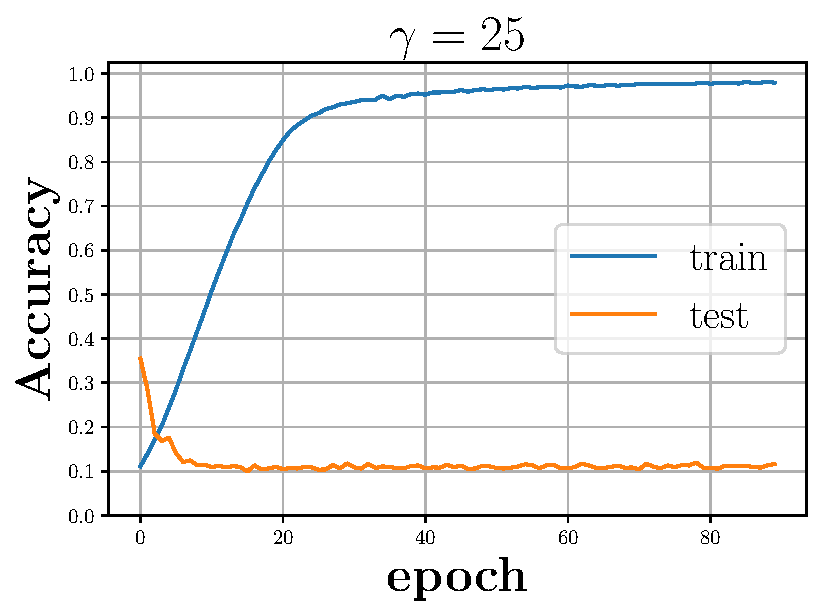
\includegraphics[scale=0.125]{figs/galu_25_bad.pdf}&
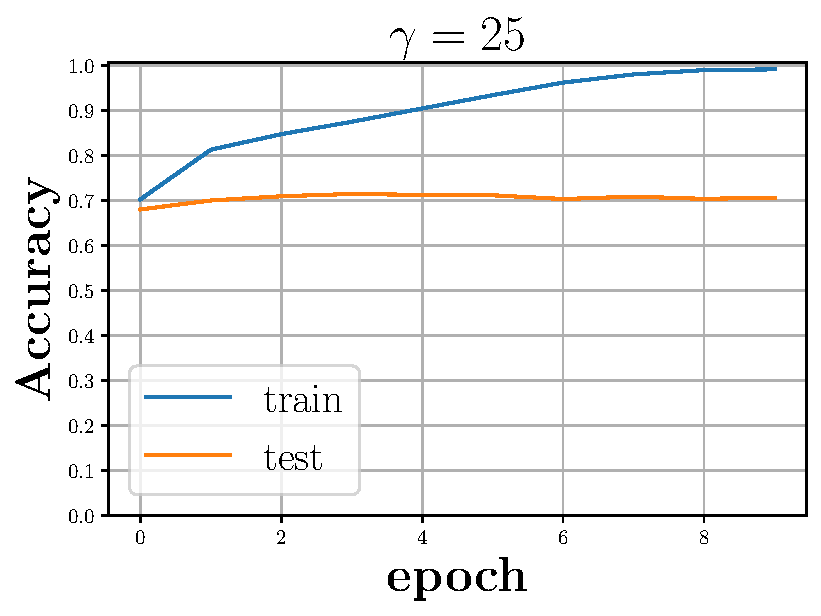
\includegraphics[scale=0.125]{figs/galu_25_bad_good.pdf}&
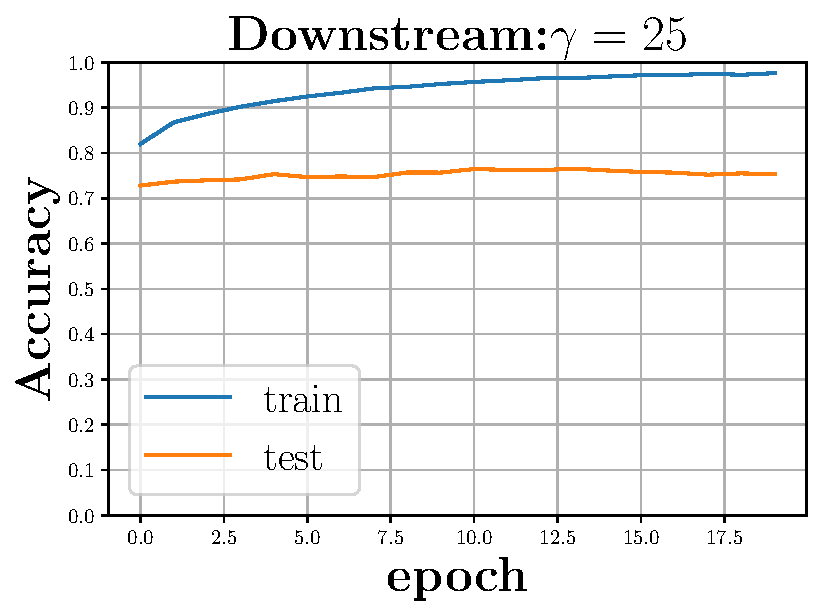
\includegraphics[scale=0.125]{figs/relu_25_good.pdf}&
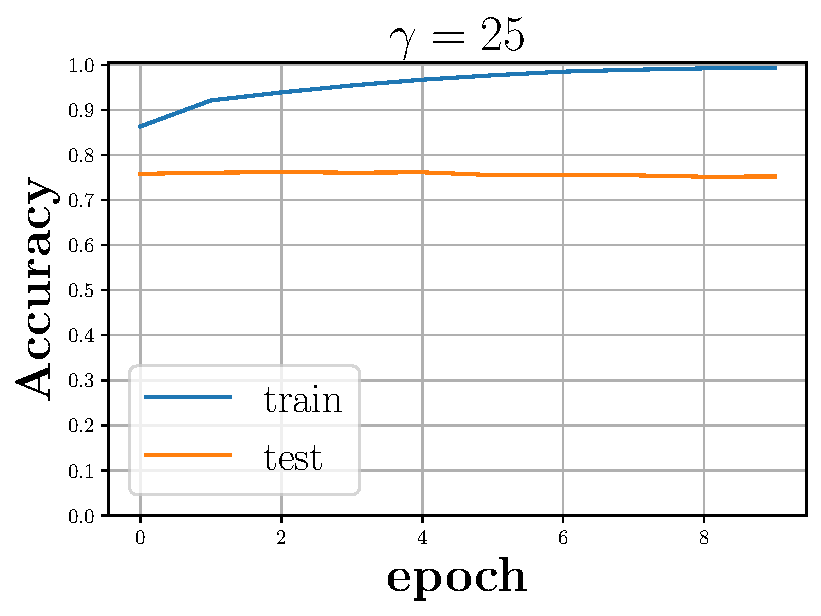
\includegraphics[scale=0.125]{figs/galu_25_recovered.pdf}
\\
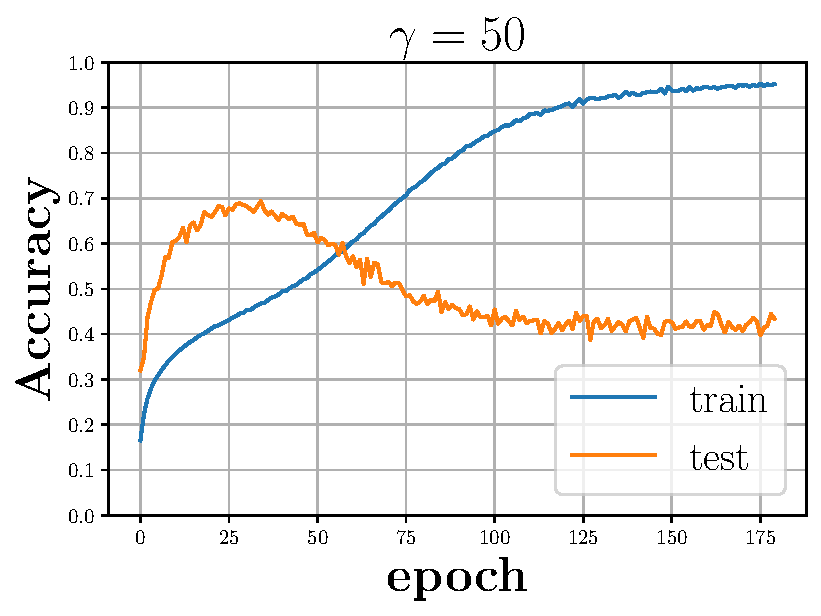
\includegraphics[scale=0.125]{figs/relu_50.pdf}&
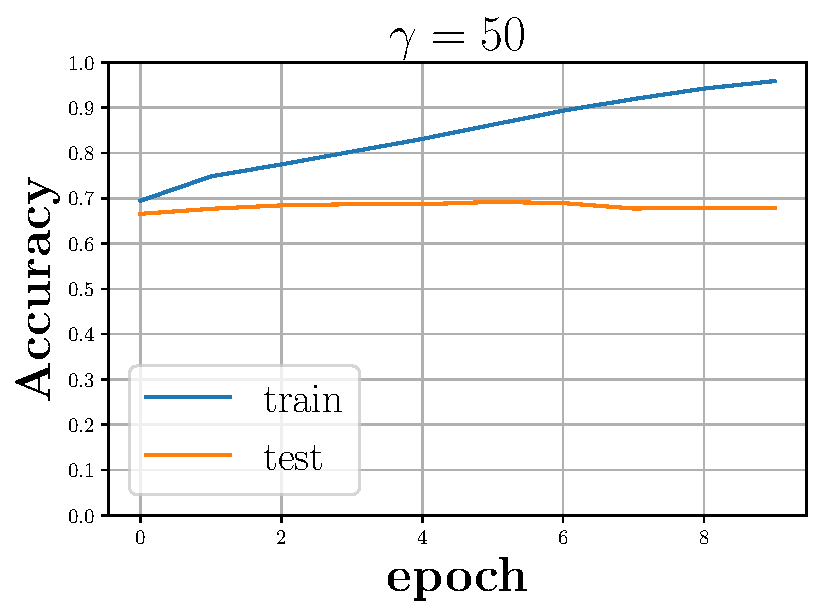
\includegraphics[scale=0.125]{figs/galu_50_good.pdf}&
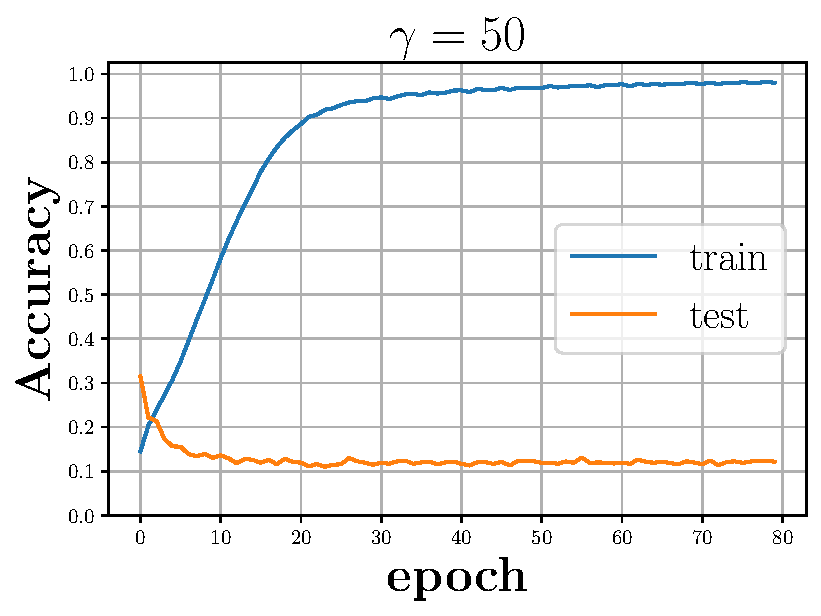
\includegraphics[scale=0.125]{figs/galu_50_bad.pdf}&
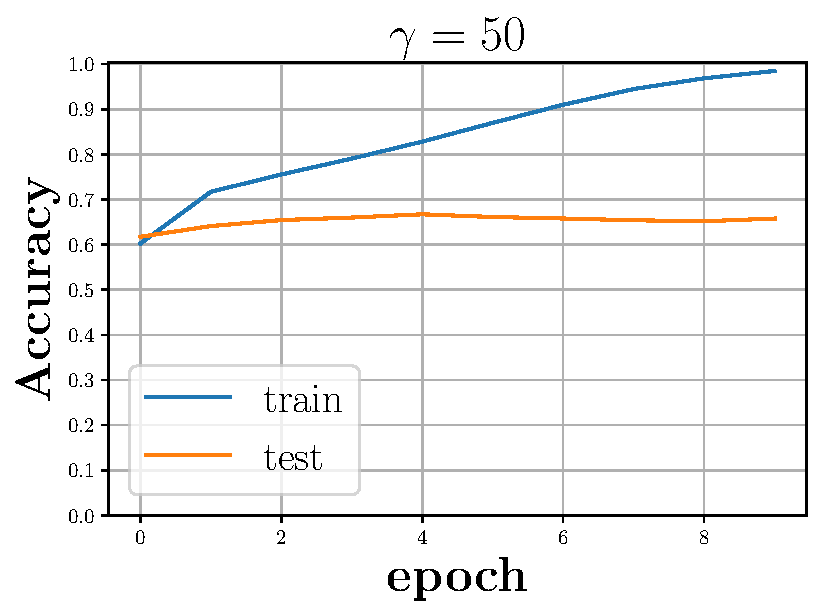
\includegraphics[scale=0.125]{figs/galu_50_bad_good.pdf}&
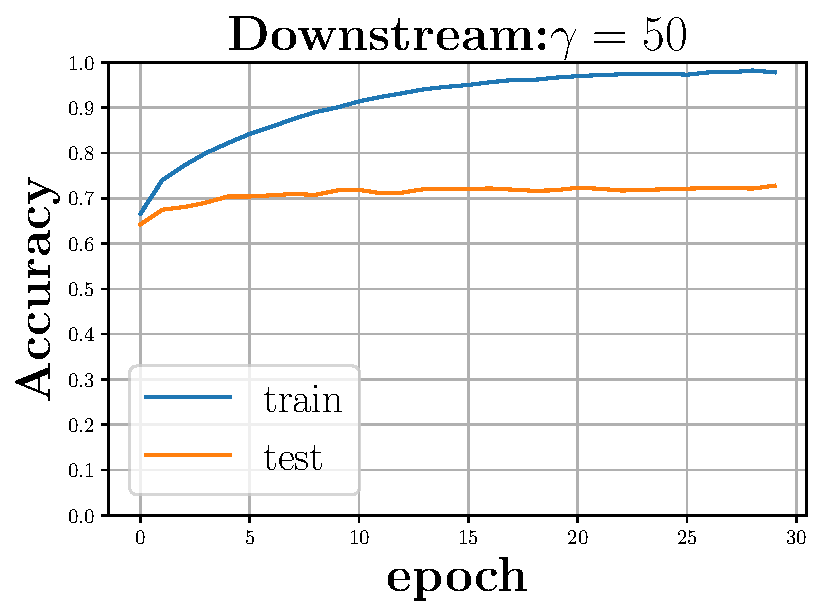
\includegraphics[scale=0.125]{figs/relu_50_good.pdf}&
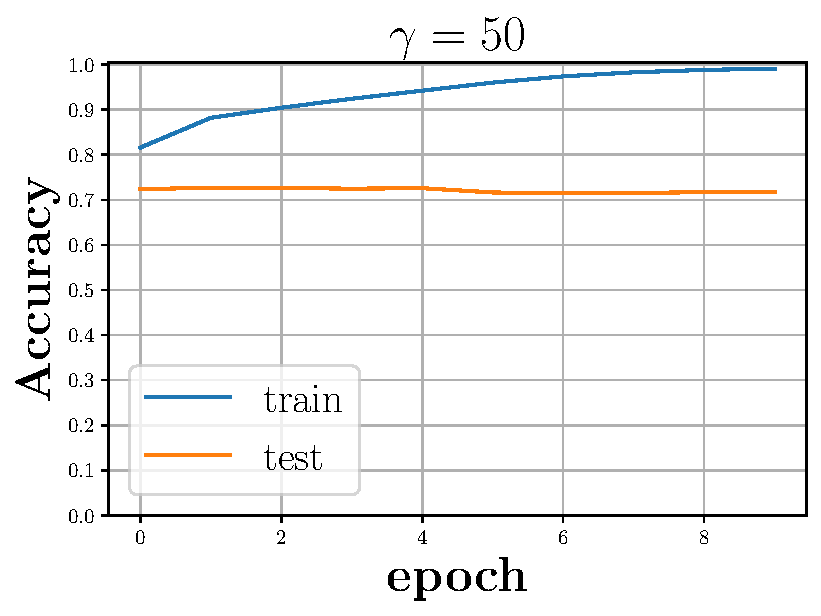
\includegraphics[scale=0.125]{figs/galu_50_recovered.pdf}
\\
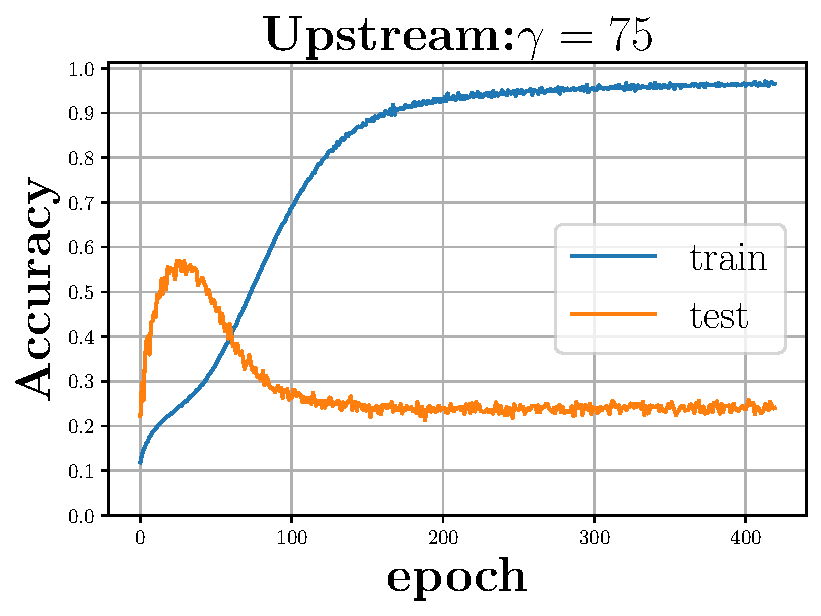
\includegraphics[scale=0.125]{figs/relu_75.pdf}&
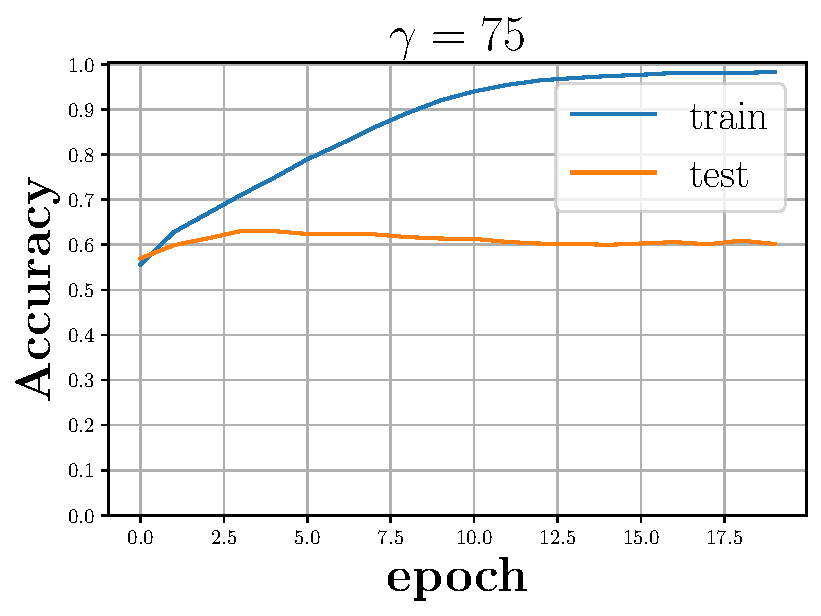
\includegraphics[scale=0.125]{figs/galu_75_good.pdf}&
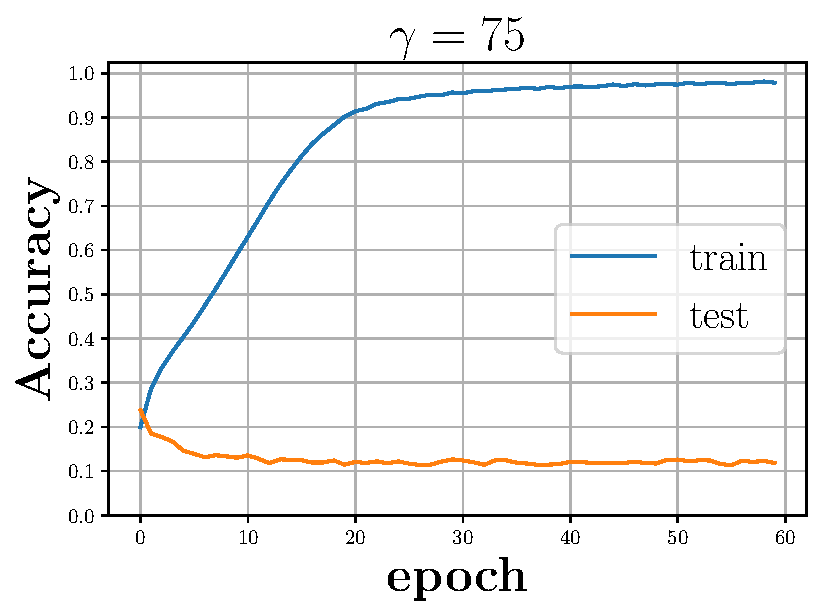
\includegraphics[scale=0.125]{figs/galu_75_bad.pdf}&
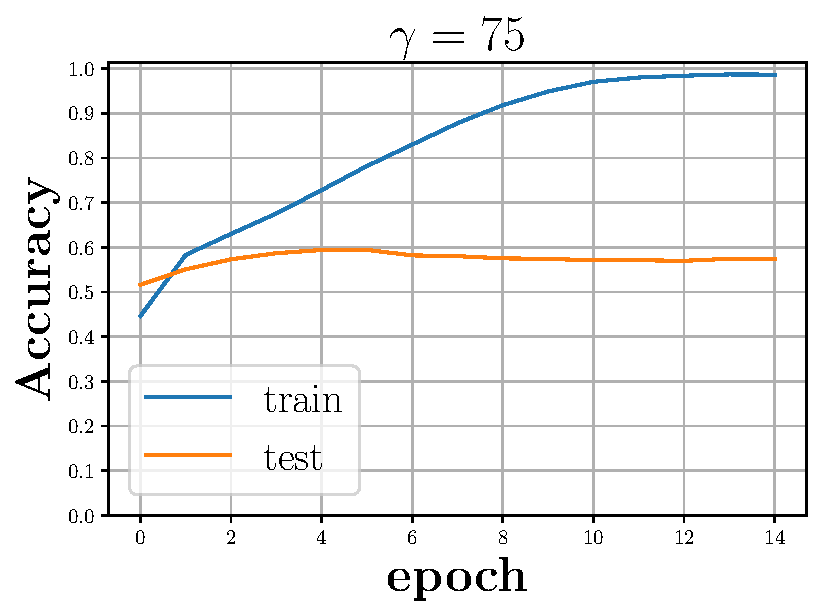
\includegraphics[scale=0.125]{figs/galu_75_bad_good.pdf}&
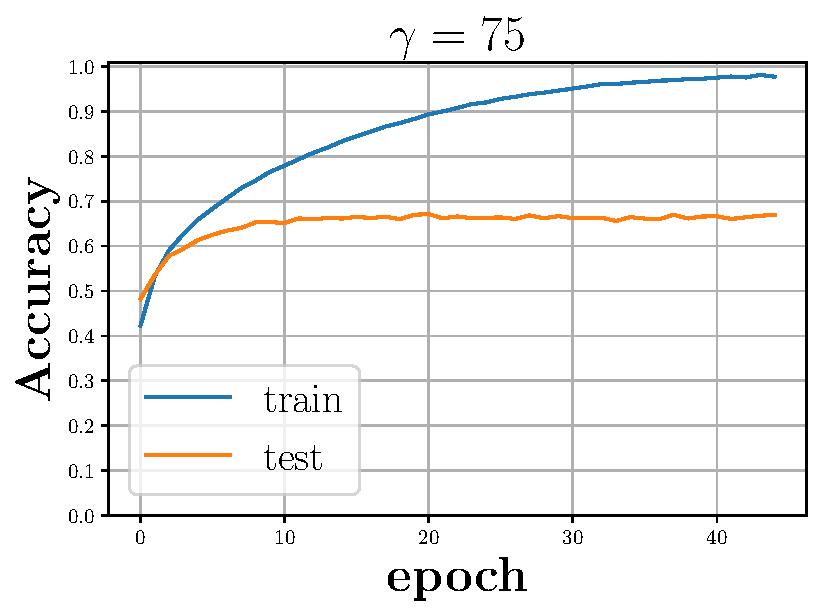
\includegraphics[scale=0.125]{figs/relu_75_good.pdf}&
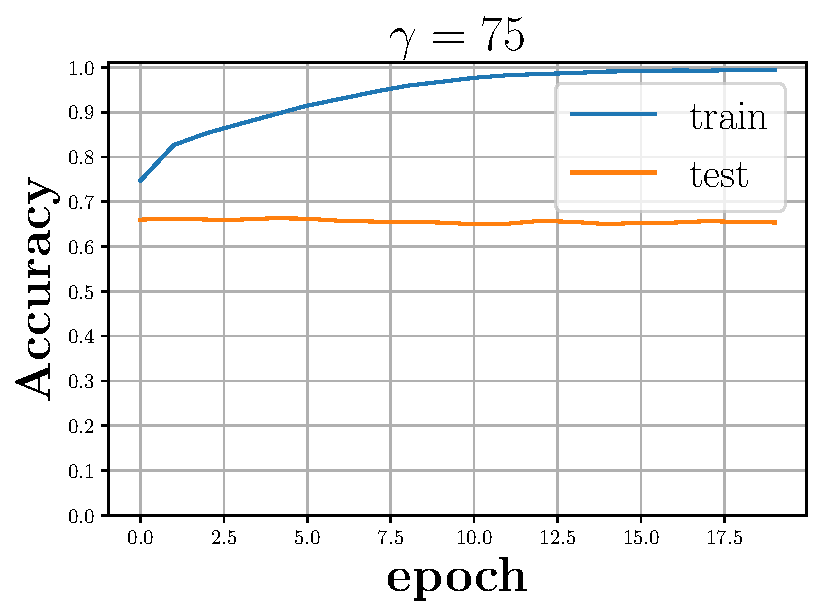
\includegraphics[scale=0.125]{figs/galu_75_recovered.pdf}\\
\tiny{M1}&\tiny{M2}&\tiny{M3:US}&\tiny{M3:DS}&\tiny{M4}&\tiny{M5}\\
\end{tabular}
}
\end{minipage}

\label{fig:rand-label}

\end{figure}

\end{comment}


\begin{comment}
\begin{figure}[h]
\begin{minipage}{0.40\columnwidth}
\begin{tabular}{|c|c|c|}\hline
ReLU& \multicolumn{2}{c|}{}\\
with   & \multicolumn{2}{c|}{Fixed Learnt Gates from }\\
 True &\multicolumn{2}{c|}{ReLU with True Labels}\\
Labels &  \multicolumn{2}{c|}{}\\\cline{2-3}
&True & {US/DS}\\\hline
 80.8& 80& 79\\\hline
 col-1 & col-2 & col-3\\\hline
\end{tabular}

\end{minipage}
\begin{minipage}{0.62\columnwidth}
\begin{tabular}{|c|c|c|c|c|c|c|c|}\hline
\%& \multicolumn{3}{c|}{\multirow{2}{*}{ReLU}} & \multicolumn{2}{c|}{FLG at End}&{FLG at End}\\
Label& \multicolumn{3}{c|}{{}} &\multicolumn{2}{c|}{of ReLU US}& of ReLU DS\\\cline{2-7}
Noise & \multicolumn{2}{c|}{Rand. US} & True & \multicolumn{1}{c|}{\multirow{2}{*}{True}} &{US/DS}& \multicolumn{1}{c|}{\multirow{2}{*}{True}} \\\cline{2-3}
{} & Best & End & DS &{} &  &\\\hline
25&75.3 & 63.1& 76.7&74.2 & 72.3& 76.5\\\hline
50& 69.8 &41.5&73.1&69.6 &67& 73.1\\\hline
 col-1 & col-2 & col-3&  col-4 & col-5 & col-6& col-7\\\hline
\end{tabular}
\end{minipage}
\end{figure}
\end{comment}

